\documentclass[11pt,a4paper]{report}

% ============================================================================
% ENCODING AND FONTS
% ============================================================================
\usepackage[utf8]{inputenc}
\usepackage[T1]{fontenc}
\usepackage{mathptmx}  % Times New Roman
\usepackage[lithuanian,english]{babel}

% ============================================================================
% PAGE LAYOUT
% ============================================================================
% Page margins: pgSz w="11906" h="16838", pgMar top="1134" right="567" bottom="1134" left="1701"
\usepackage[top=2.00cm, right=1.00cm, bottom=2.00cm, left=3.00cm, headheight=1.0cm, headsep=1.0cm, footskip=1.0cm]{geometry}

% ============================================================================
% GRAPHICS AND FIGURES
% ============================================================================
\usepackage{graphicx}
\usepackage{booktabs}
\usepackage{svg}
\svgsetup{inkscapelatex=false}
\usepackage{float}
\usepackage[labelfont={bf,it}, labelsep=period]{caption}
\captionsetup[figure]{labelformat=simple, textfont=it}

% ============================================================================
% COLORS
% ============================================================================
\usepackage{xcolor}

% ============================================================================
% TEXT FORMATTING
% ============================================================================
\usepackage{setspace}
\usepackage{parskip}
\usepackage{indentfirst}
\usepackage{titlesec}
\usepackage{fancyhdr}

% ============================================================================
% HYPERLINKS (load before cleveref)
% ============================================================================
\usepackage[breaklinks=true]{hyperref}
\hypersetup{
    colorlinks=true,
    urlcolor=blue,
    linkcolor=black,
    citecolor=black
}
\urlstyle{same}

% ============================================================================
% CROSS-REFERENCES (must load after hyperref)
% ============================================================================
\usepackage[nameinlink,noabbrev]{cleveref}

% Figure references: "fig.1", "Fig.1", "figs.1–3", no brackets
\crefname{figure}{fig.}{figs.}
\Crefname{figure}{Fig.}{Figs.}

% ============================================================================
% CODE LISTINGS
% ============================================================================
\let\origttdefault\ttdefault
\usepackage[scaled=1.1]{beramono}
\renewcommand{\ttdefault}{\origttdefault}  % Restore document-wide monospace

\usepackage{fancyvrb}
\RecustomVerbatimEnvironment{verbatim}{Verbatim}{%
    frame=single,
    framerule=0.8pt,
    fontsize=\small,
    xleftmargin=4pt,
    xrightmargin=4pt
}

\usepackage{listings}

\lstset{
    basicstyle=\fontfamily{fvm}\selectfont\footnotesize,  % Beramono only here
    keywordstyle=\color{blue},
    stringstyle=\color{olive},
    commentstyle=\color{gray},
    identifierstyle=\color{black},
    numbers=left,
    numberstyle=\tiny\color{gray},
    stepnumber=1,
    numbersep=8pt,
    showstringspaces=false,
    breaklines=true,
    keepspaces=true,
    frame=single,
    framerule=0.4pt,
    rulecolor=\color{black},
    backgroundcolor=\color{white},
    captionpos=b,
    language=C++
}

% ============================================================================
% SPACING AND PARAGRAPH SETTINGS
% ============================================================================
% Line spacing: Normal style line="360" = 360/240 = 1.5
\setstretch{1.5}
\setlength{\parindent}{36pt}
\setlength{\parskip}{6pt}
\emergencystretch=2em

% ============================================================================
% DOCUMENT METADATA
% ============================================================================
% Title page content - modify these as needed

\newcommand{\ttinline}[1]{\mbox{\texttt{#1}}}

% ============================================================================
% PAGE STYLE AND HEADERS
% ============================================================================
% Title page has no page numbers (page break after title page in Word)
\pagestyle{empty}

% Headers and footers for main document
\fancyhf{}
\renewcommand{\headrulewidth}{0pt}
\renewcommand{\footrulewidth}{0pt}

% ============================================================================
% SECTION NUMBERING AND FORMATTING
% ============================================================================
% Enable numbering for subsubsections (LaTeX default only numbers up to subsection level)
\setcounter{secnumdepth}{3}  % 0=chapter, 1=section, 2=subsection, 3=subsubsection

% Section numbering: sections start from 1., subsections are 1.x, subsubsections are 1.x.x.
\renewcommand{\thesection}{\arabic{section}.}
\renewcommand{\thesubsection}{\arabic{section}.\arabic{subsection}}
\renewcommand{\thesubsubsection}{\arabic{section}.\arabic{subsection}.\arabic{subsubsection}.}

% Chapter and section formatting - hierarchical indentation with smaller increments
\titleformat{\chapter}[block]
    {\normalfont\fontsize{14}{16.8}\selectfont\bfseries}
    {\thechapter}
    {1em}
    {}  % BDSkyrius1lygio: sz="28"=14pt
\titlespacing*{\chapter}{0pt}{*2}{*2}

\titleformat{\section}[block]
    {\normalfont\fontsize{12}{18}\selectfont\bfseries}
    {\thesection}
    {1em}
    {}  % BDSkyrius1lygio: no indentation
\titlespacing*{\section}{0pt}{*1.5}{*1}

\titleformat{\subsection}[block]
    {\normalfont\fontsize{12}{18}\selectfont\bfseries}
    {\hspace{20pt}\thesubsection}
    {1em}
    {}  % BDSkyrius2lygio: 20pt indent
\titlespacing*{\subsection}{0pt}{*1.2}{*0.8}

\titleformat{\subsubsection}[block]
    {\normalfont\normalsize\itshape}
    {\hspace{40pt}\thesubsubsection}
    {1em}
    {}  % BDSkyrius3lygio: 40pt indent (progressive)
\titlespacing*{\subsubsection}{0pt}{*1}{*0.6}

% ============================================================================
% DOCUMENT BODY
% ============================================================================
\begin{document}

% Create title page
\begin{titlepage}
    \centering

    % University logo
    
\includegraphics[width=4.92cm]{images/vgtu_logo.png}

    % University name (14pt, uppercase, no bold)
    {\fontsize{14}{21}\selectfont\MakeUppercase{VILNius gediminas technical university}}

    % Faculty (12pt, uppercase)
    {\fontsize{12}{18}\selectfont\MakeUppercase{faculty of fundamental sciences}}

    % Department (12pt, uppercase)
    {\fontsize{12}{18}\selectfont\MakeUppercase{department of information technologies}}

    \vspace{84pt}

    % Student name (14pt, normal case)
    {\fontsize{14}{21}\selectfont Elvinas Žukauskas}

    \vspace{30pt}

    % Thesis title Lithuanian (14pt, bold, uppercase)
    {\fontsize{14}{21}\selectfont\bfseries\MakeUppercase{Android vietinių funkcijų perėmimas šifruotoms bibliotekoms}}

    % Thesis title English (14pt, bold, uppercase)
    {\fontsize{14}{21}\selectfont\bfseries\MakeUppercase{Android native call hooking for encrypted libraries}}

    \vspace{60pt}

    % Work type (14pt, normal)
    {\fontsize{14}{21}\selectfont Final Bachelor Thesis}

    \vspace{30pt}

    % Study program (12pt, normal)
    {\fontsize{12}{18}\selectfont Engineering Informatics Study Programme, State code 6121BX033}

    % Specialization (12pt, normal)
    {\fontsize{12}{18}\selectfont Informacinių technologijų valdymo specialization}

    % Study field (12pt, normal)
    {\fontsize{12}{18}\selectfont Study Field of Informatics}

    \vspace{168pt}

    % Year and city (12pt, normal)
    {\fontsize{12}{18}\selectfont Vilnius, 2026}

\end{titlepage}
\newpage

% Create second page (Lithuanian approval page)
\begin{titlepage}
    \centering

    % University / faculty / department (centered, uppercase)
    {\large\MakeUppercase{VILNIAUS GEDIMINO TECHNIKOS UNIVERSITETAS}\\}
    {\normalsize\MakeUppercase{Fundamentinių mokslų fakultetas}\\}
    {\normalsize\MakeUppercase{Informacinių technologijų katedra}\\}

    \vspace{1cm}

    % PATVIRTINTA block (right-aligned)
    \begin{flushright}
        \small
        PATVIRTINTA \\
        Katedros vedėjo \\
        doc. dr. Dmitrij Šešok
    \end{flushright}

    \vspace{2cm}

    % Student name
    \normalsize
    Elvinas Žukauskas

    \vspace{1cm}

    % Lithuanian and English titles (bold, uppercase)
    \large
    \textbf{\MakeUppercase{Android vietinių funkcijų perėmimas šifruotoms bibliotekoms}}\\[0.5cm]
    \textbf{\MakeUppercase{Android native call hooking for encrypted libraries}}

    \vspace{2cm}

    % Work type
    \large
    Baigiamasis bakalauro darbas

    \vspace{2cm}

    % Study program / specialization / field (Lithuanian)
    \normalsize
    Inžinerinės informatikos studijų programa, valstybinis kodas 6121BX033 \\
    Informacinių technologijų valdymo specializacija \\
    Informatikos studijų kryptis

    \vspace{2.5cm}

    % Supervisors (no box, right aligned)
    \begin{flushright}
        \normalsize
        \textbf{Vadovas} doc. dr. Saulius Valentinavičius\\
        {\tiny (Pedag. vardas, vardas, pavardė)}\\[0.8cm]
    \end{flushright}

    \vfill

    % City and year at the bottom
    \normalsize
    Vilnius, 2026

\end{titlepage}
\newpage

% Switch to main document formatting for subsequent pages
\pagestyle{plain}
\pagenumbering{arabic}
\setcounter{page}{3}  % Start page numbering from 3 as in the docx

\setcounter{tocdepth}{3}
\tableofcontents
\newpage

% ============================================================================
% INTRODUCTION
% ============================================================================
\section*{Introduction}
\addcontentsline{toc}{section}{Introduction}

\textbf{Relevance of the thesis.} Intellectual property protection has long been a focus in the field of cybersecurity. On mobile platforms such as Android, one important aspect of this protection is encrypting native libraries and ensuring that they are only decrypted at runtime. While this can be achieved easily when a native library is loaded from Java, a greater challenge arises when native libraries load other native libraries. This issue is particularly relevant in cross-platform frameworks such as Flutter (used in approximately 11\% of Android apps~\cite{appfigures2024flutter}) and .NET MAUI, which provide a single codebase across multiple targets but internally depend on platform-specific mechanisms, including cases where native libraries load other native libraries. Such nested loading scenarios complicate protection processes, as traditional Java-based hooking approaches do not address native loading calls. Addressing these challenges is crucial for maintaining the confidentiality and integrity of sensitive application components in modern mobile ecosystems.

\textbf{Problem of the thesis.} Existing protection mechanisms do not address scenarios where native libraries load other native libraries, leaving such cases vulnerable to unauthorized access. This thesis proposes and implements a proof-of-concept solution that intercepts Android native library loading calls and replaces them with custom logic to decrypt libraries before they are loaded, thereby extending protection beyond standard Java-based loading mechanisms.

\textbf{Objective of the thesis:} Research possible solutions for intercepting Android native loading calls and developing a proof-of-concept implementation.

\textbf{Tasks of the thesis:}
\begin{enumerate}
    \item Analyze native library loading mechanisms in Android.
    \item Examine and evaluate techniques for intercepting native loading calls.
    \item Design a proof-of-concept architecture for custom interception and decryption.
    \item Implement and test the proof-of-concept solution.
\end{enumerate}

\newpage

% ============================================================================
% MAIN CONTENT
% ============================================================================
\section{Analysis and Overview of Relevant Technologies}

Android provides the runtime environment in which the proof-of-concept system operates.  It manages hardware access, memory, process isolation, and security for every installed application.  Developers typically target Android through the Software Development Kit (SDK), which supplies high-level APIs for user interfaces, data management, and system-service interaction across different devices and OS versions.

When SDK-level code is insufficient, such as when reusing an existing C library or meeting strict latency requirements, the Native Development Kit (NDK) allows developers to compile C and C++ code into shared objects that run inside an application process.  The NDK bridges managed and native layers and is central to the library-loading mechanism this thesis intercepts.

Hooking (function interception) is the technique of redirecting control flow at runtime to observe or modify a program's behaviour without changing its source code.  Security researchers use it for monitoring and debugging; attackers use the same mechanisms to bypass protections or manipulate application logic.  This dual nature makes hooking both the tool and the threat model in this thesis.

Encryption transforms data into an unreadable form; decryption reverses the transformation when the correct key is available.  Applied to native libraries, encryption can ensure that an \texttt{.so} file stored on disk is useless to an attacker who lacks the key.  Combined with controlled interception of the loading path, encrypted libraries can be restored to a loadable state only at the moment they are needed, within the memory of the authorised process.

\subsection{Android Platform}
\subsubsection{Platform Architecture}

As shown in \cref{fig:android_software_stack}, Android is structured as a layered software stack built on a modified Linux kernel. The kernel provides essential system services, such as process and memory management, drivers, networking, and security mechanisms. \cite{android_platform}

\begin{figure}[p]
    \centering
    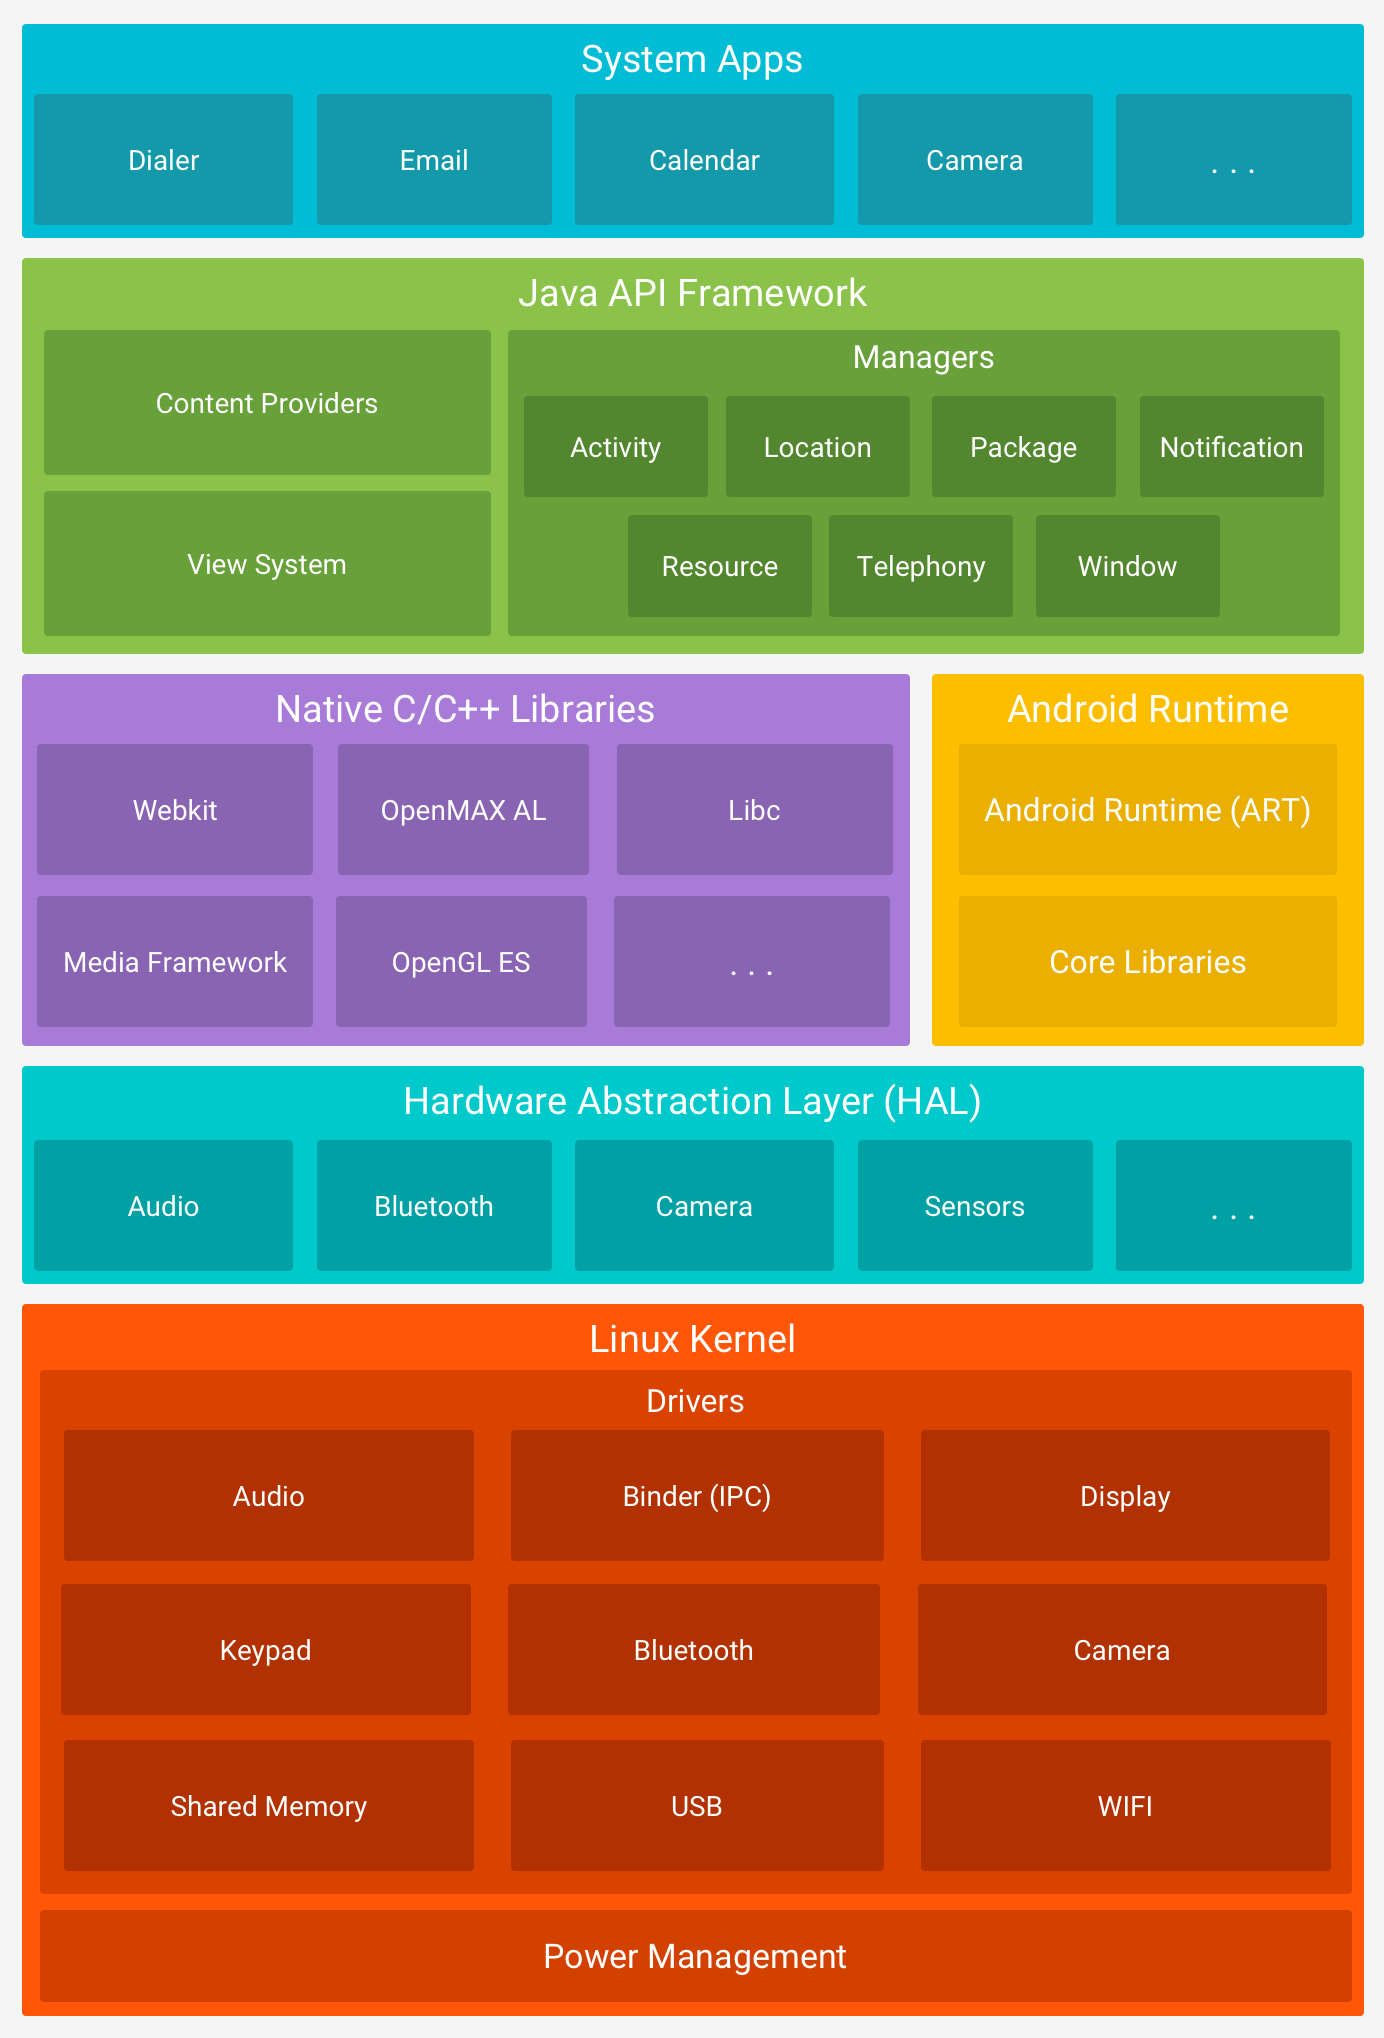
\includegraphics[width=0.8\textwidth]{images/android_software_stack.png}
    \caption{The Android software stack. \cite{android_platform}}
    \label{fig:android_software_stack}
\end{figure}

Above the kernel is the Hardware Abstraction Layer (HAL), which defines standardized interfaces that enable higher layers of the system to communicate with device-specific hardware components. The next layer consists of native C/C++ libraries and the Android Runtime (ART). These native libraries provide system-level functionality for areas such as graphics, media, and databases. ART executes application bytecode and is responsible for ahead-of-time (AOT) and just-in-time (JIT) compilation, garbage collection, and debugging support. On top of this layer is the Java application programming interface (API) framework, which exposes system features to applications through objects, services, and APIs. This layer simplifies access to device capabilities and system services for application developers. The highest layer contains applications, including both system-installed and user-installed apps. Each application runs in its own process and interacts with the Java API framework to utilize the underlying system functionality. \cite{android_platform}

\subsubsection{Native Libraries in Android}

Native libraries in Android are shared C/C++ libraries compiled into \texttt{.so} files. They extend application functionality beyond the Java or Kotlin layer, enabling performance critical operations and access to low level system features. These libraries are packaged inside the application under the \texttt{lib/<ABI>/} directories, with separate binaries for each supported processor architecture, such as \texttt{armeabi-v7a}, \texttt{arm64-v8a}, or \texttt{x86\_64}.

Native code interacts with the managed environment through the Java Native Interface (JNI). JNI is a standardized framework that enables interoperability between managed Java code and unmanaged native code written in C or C++. It allows Java applications to invoke native functions for performance critical tasks, system level operations, or to reuse existing native codebases. It also permits native code to call back into Java, creating a bidirectional communication channel between the Android Runtime (ART) and compiled native libraries.

A typical JNI workflow is illustrated in \cref{fig:jni_workflow_mermaid}. At a high level, the application declares one or more methods as \texttt{native} in the Java or Kotlin layer, requests loading of the corresponding shared library via \texttt{System.loadLibrary()}, and relies on ART and JNI to bind these declarations to concrete functions in the native library. After the library is loaded, calls from managed code to the native methods are routed through the JNI bridge to the compiled C or C++ implementation, which can then interact with Java objects through the \texttt{JNIEnv*} interface and return data back to the managed layer.

\begin{figure}[p]
    \centering
    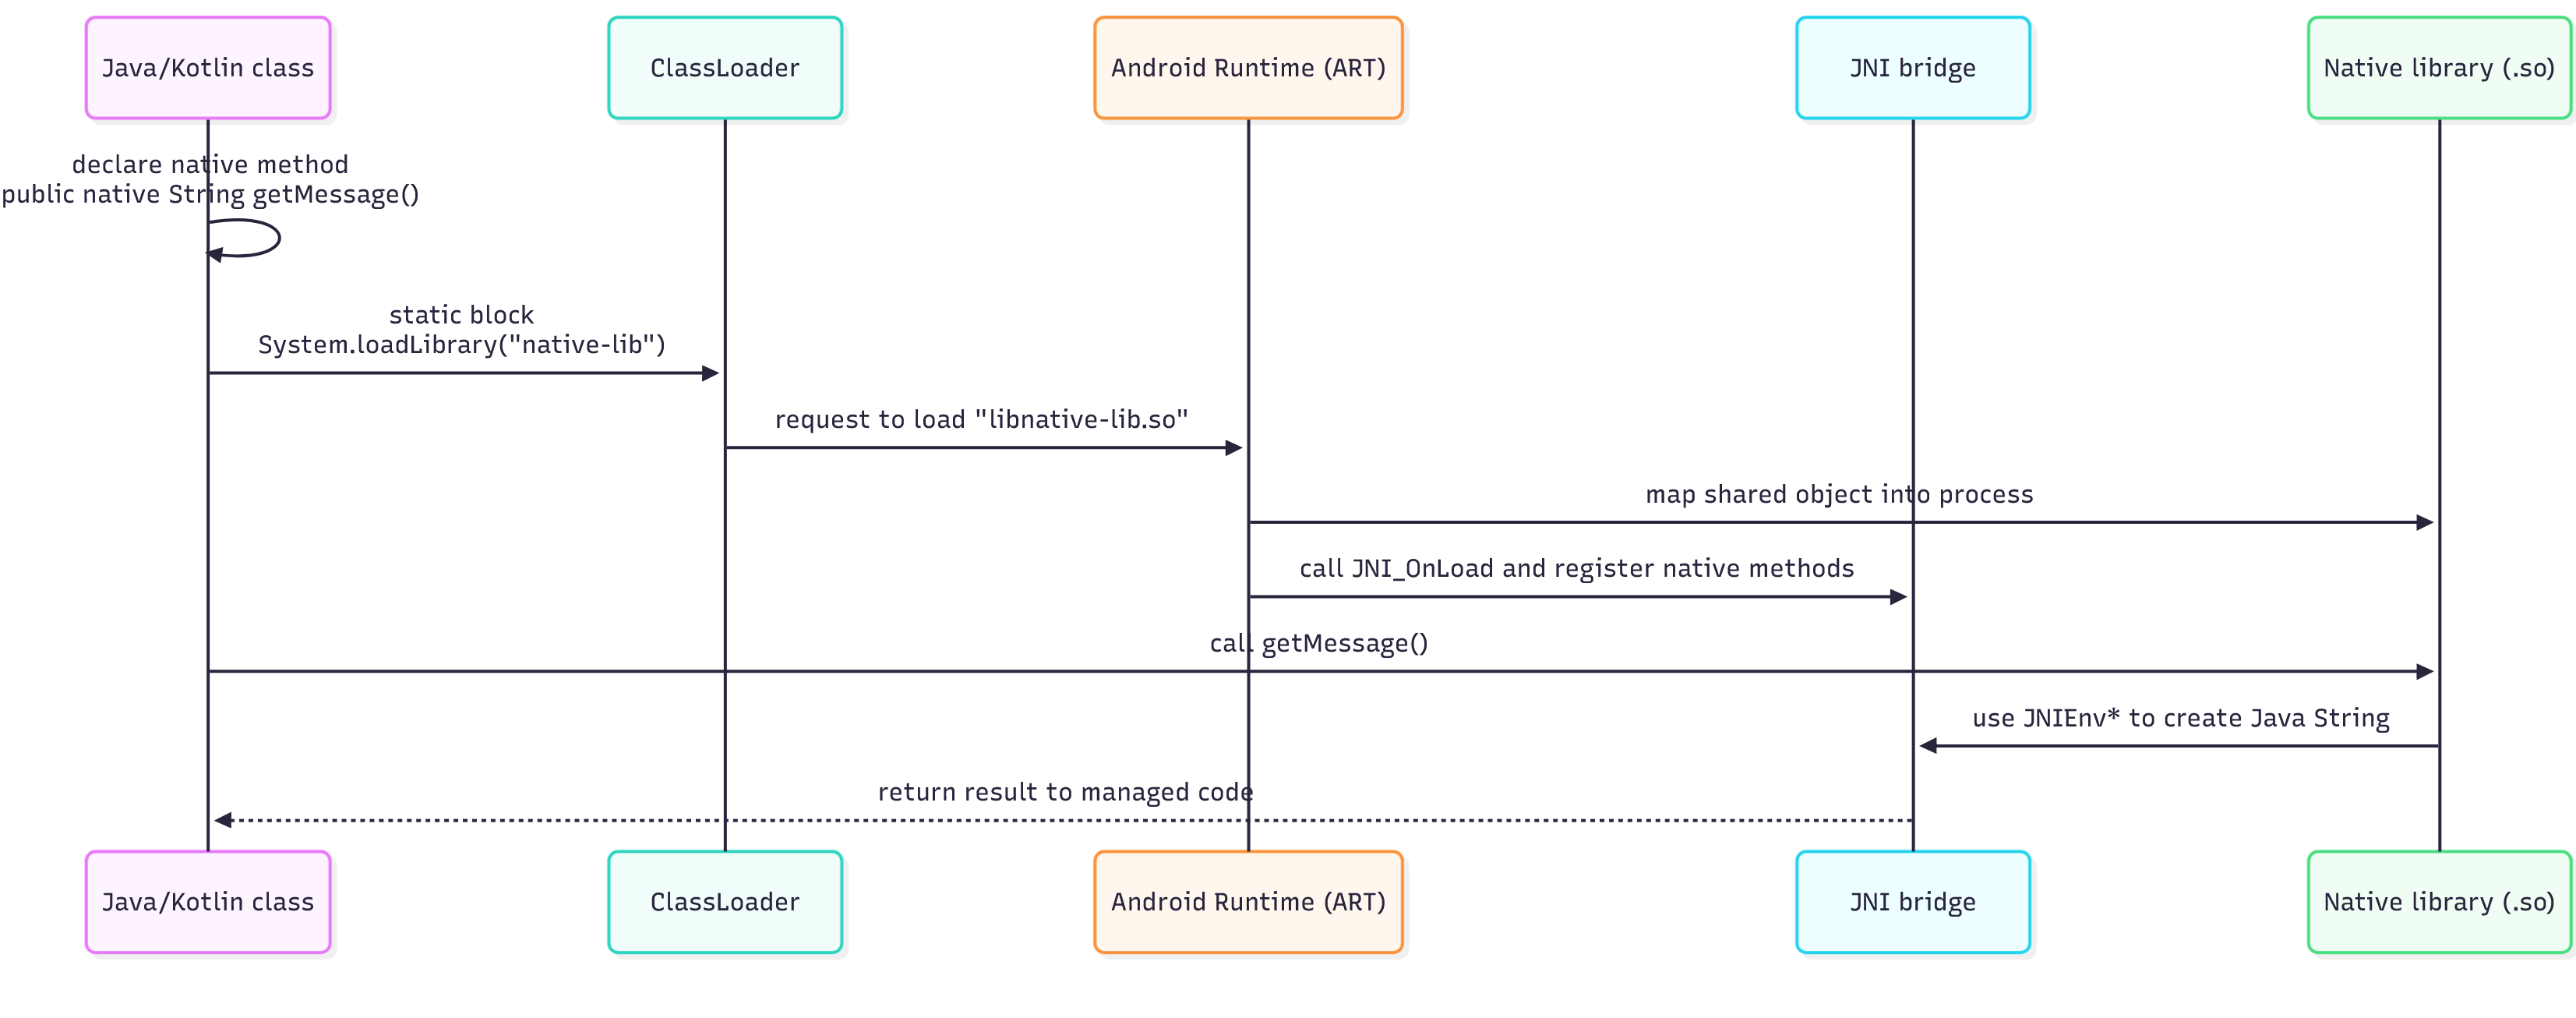
\includegraphics[width=1\textwidth]{images/java_class_declaring_native_method.png}
    \caption{High level JNI workflow between Java and native layers.}
    \label{fig:jni_workflow_mermaid}
\end{figure}

The \texttt{JNIEnv*} interface exposed to native code provides access to the managed environment, including operations such as creating new Java strings, invoking Java methods, or managing exceptions. JNI therefore serves as the fundamental bridge between Android managed and native layers, allowing developers to balance execution speed, resource control, and portability when building hybrid applications that combine both Java and C/C++ code.

\subsubsection{ELF Format and Dynamic Linking on Android}

Android native libraries are distributed as shared objects with the \texttt{.so} extension. These binaries follow the Executable and Linkable Format (ELF), which is the standard binary format for Linux based systems, including Android. ELF defines how code, data, and metadata are organized so that the operating system and the dynamic linker can map the library into memory and resolve its dependencies at runtime \cite{xinuos2025elf}.

As shown in \cref{fig:elf_link_exec_views}, an ELF shared object is organized in terms of sections and segments. The linker oriented view groups code and data into sections and records them in the Section Header Table, which is mainly used for linking and static analysis. The loader oriented view groups data into loadable segments that are described by the Program Header Table. Loadable segments contain executable code and data that are mapped directly into a process address space. Metadata sections describe symbols, relocations, dependencies, and initialization logic. Of particular importance for dynamic loading are the dynamic symbol table, relocation entries, and the \texttt{.init\_array} constructors. These elements allow the loader to connect the library to the rest of the process at runtime without recompiling the application \cite{xinuos2025elf}.

\begin{figure}[p]
    \centering
    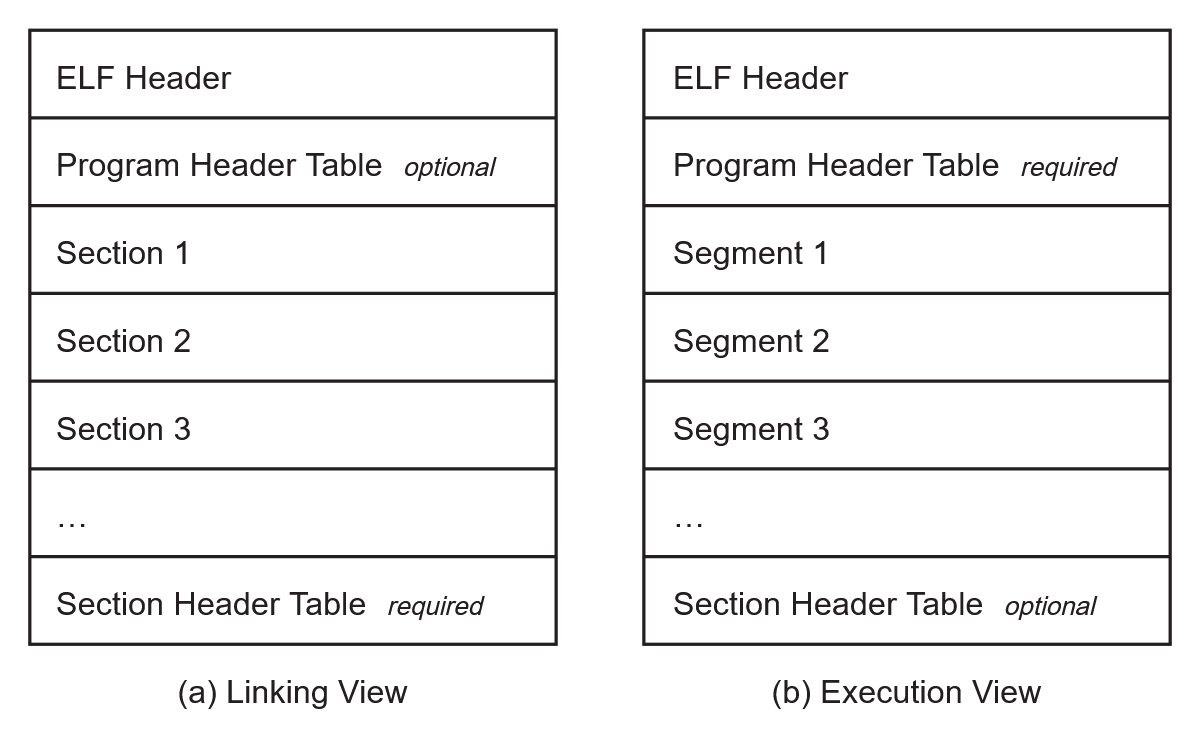
\includegraphics[width=0.625\textwidth]{images/elf_link_exec_views.png}
    \caption{Structure of an ELF shared object: (a) linking view; (b) execution view. Adapted from the System V Application Binary Interface ELF specification \cite{xinuos2025elf}.}
    \label{fig:elf_link_exec_views}
\end{figure}

External function calls in ELF are typically resolved through two related structures: the Procedure Linkage Table (PLT) and the Global Offset Table (GOT). Calls to functions provided by other libraries are compiled as indirect jumps through the PLT. At runtime the PLT consults the GOT, which holds the resolved addresses of external symbols. During loading, the dynamic linker updates GOT entries so that subsequent calls jump directly to the correct target function. Because this indirection is based on tables of function pointers, native hooking techniques often modify or replace those resolved entries after load in order to redirect execution flow \cite{ronin2018hooking}.

The ELF format also encodes library dependencies using entries in the \texttt{DT\_NEEDED} list. Each \texttt{DT\_NEEDED} record names another shared object that must be available for correct execution. When a library is loaded, the Android dynamic linker inspects these entries, locates the required dependencies, and loads them into memory if they are not already present. The linker then performs relocations, which are adjustments that patch absolute and relative addresses in code and data so that all symbol references point to the correct locations in the current process image. After relocations are applied, external calls through the PLT and GOT resolve to valid function addresses \cite{xinuos2025elf}.

After mapping segments and applying relocations, the loader executes any registered initialization routines. On Android this includes running functions listed in the \texttt{.init\_array} section and invoking the optional \texttt{JNI\_OnLoad} entry point if the library is intended to be used through the Java Native Interface (JNI). The \texttt{JNI\_OnLoad} function is called once when the library is first attached to the Java environment. It typically registers native methods with the Android Runtime (ART) so that managed code can invoke them. This registration step links method signatures in Java to concrete function pointers in the loaded ELF binary \cite{xinuos2025elf,bleier2023oat}.

Modern versions of Android also enforce linker namespaces. A namespace defines which libraries are visible to a given loading context and which symbols can be resolved across boundaries. Application code, system libraries, and vendor components may reside in separate namespaces. This separation limits access to private system interfaces and prevents accidental or unauthorized linking against internal libraries. It also means that two libraries with the same filename can coexist in different namespaces, and it affects whether repeated loading of the same \texttt{.so} is permitted under different class loaders.

In summary, the ELF format provides the structural basis for how Android represents native code, and the dynamic linker is responsible for locating dependencies, applying relocations, resolving symbols through PLT and GOT, and invoking initialization code. These mechanisms are also the points at which native level interception can observe or redirect operations such as \texttt{dlopen()}, symbol resolution, or library initialization. This makes ELF level behavior directly relevant to runtime decryption and controlled loading of protected libraries \cite{xinuos2025elf,ronin2018hooking,bleier2023oat}.

\subsubsection{Library Loading Mechanisms}

Android provides multiple ways to load native libraries at runtime. The most common method is Java-based loading through \texttt{System.load()} and \texttt{System.loadLibrary()}, which delegate the work to the Android Runtime (ART) and the process linker (the bionic linker). These functions locate, validate, map, and initialize the requested shared object (\texttt{.so}) file.

\cref{fig:android_lib_load_flow} illustrates the high-level flow used when an application calls \texttt{System.loadLibrary("foo")} or \texttt{System.load("/abs/path/libfoo.so")}. The class loader first resolves the requested library name to an absolute filesystem path. ART then performs several checks before loading the library, including verifying whether the same library has already been loaded for the same \texttt{ClassLoader}. If the library is already associated with that \texttt{ClassLoader}, the call returns successfully without reloading it.

However, if the library is already loaded in a \emph{different} \texttt{ClassLoader}, ART rejects the load and reports an \texttt{UnsatisfiedLinkError}. This prevents the same binary from being linked into multiple class loader namespaces in the same process.

If the load proceeds, ART delegates to the bionic linker, which applies normal ELF loading semantics. The linker locates the library in the namespaces and search paths associated with the calling \texttt{ClassLoader}. It then maps the ELF segments into memory, resolves \texttt{DT\_NEEDED} dependencies according to that namespace's visibility rules, and applies relocations. After that, it runs constructor sections (such as \texttt{.init\_array}) and finally calls the library's optional \texttt{JNI\_OnLoad} entry point. During \texttt{JNI\_OnLoad}, the library usually registers its native methods with the runtime. ART then records the handle of the loaded library and associates it with the calling \texttt{ClassLoader} for future lookups.

In addition to Java-based loading, libraries can also be loaded directly from native code using \texttt{dlopen()} without going through \texttt{System.loadLibrary()}. In that case, the library is opened by the dynamic linker from C/C++ code, and the Java side may never see it as part of a \texttt{ClassLoader}. This pattern is widely used in engine-style code and multilayer runtimes, including cross-platform frameworks such as Flutter and .NET MAUI, where one native component loads and binds another at runtime using only the POSIX-level dynamic loading API.

\begin{figure}[p]
    \centering
    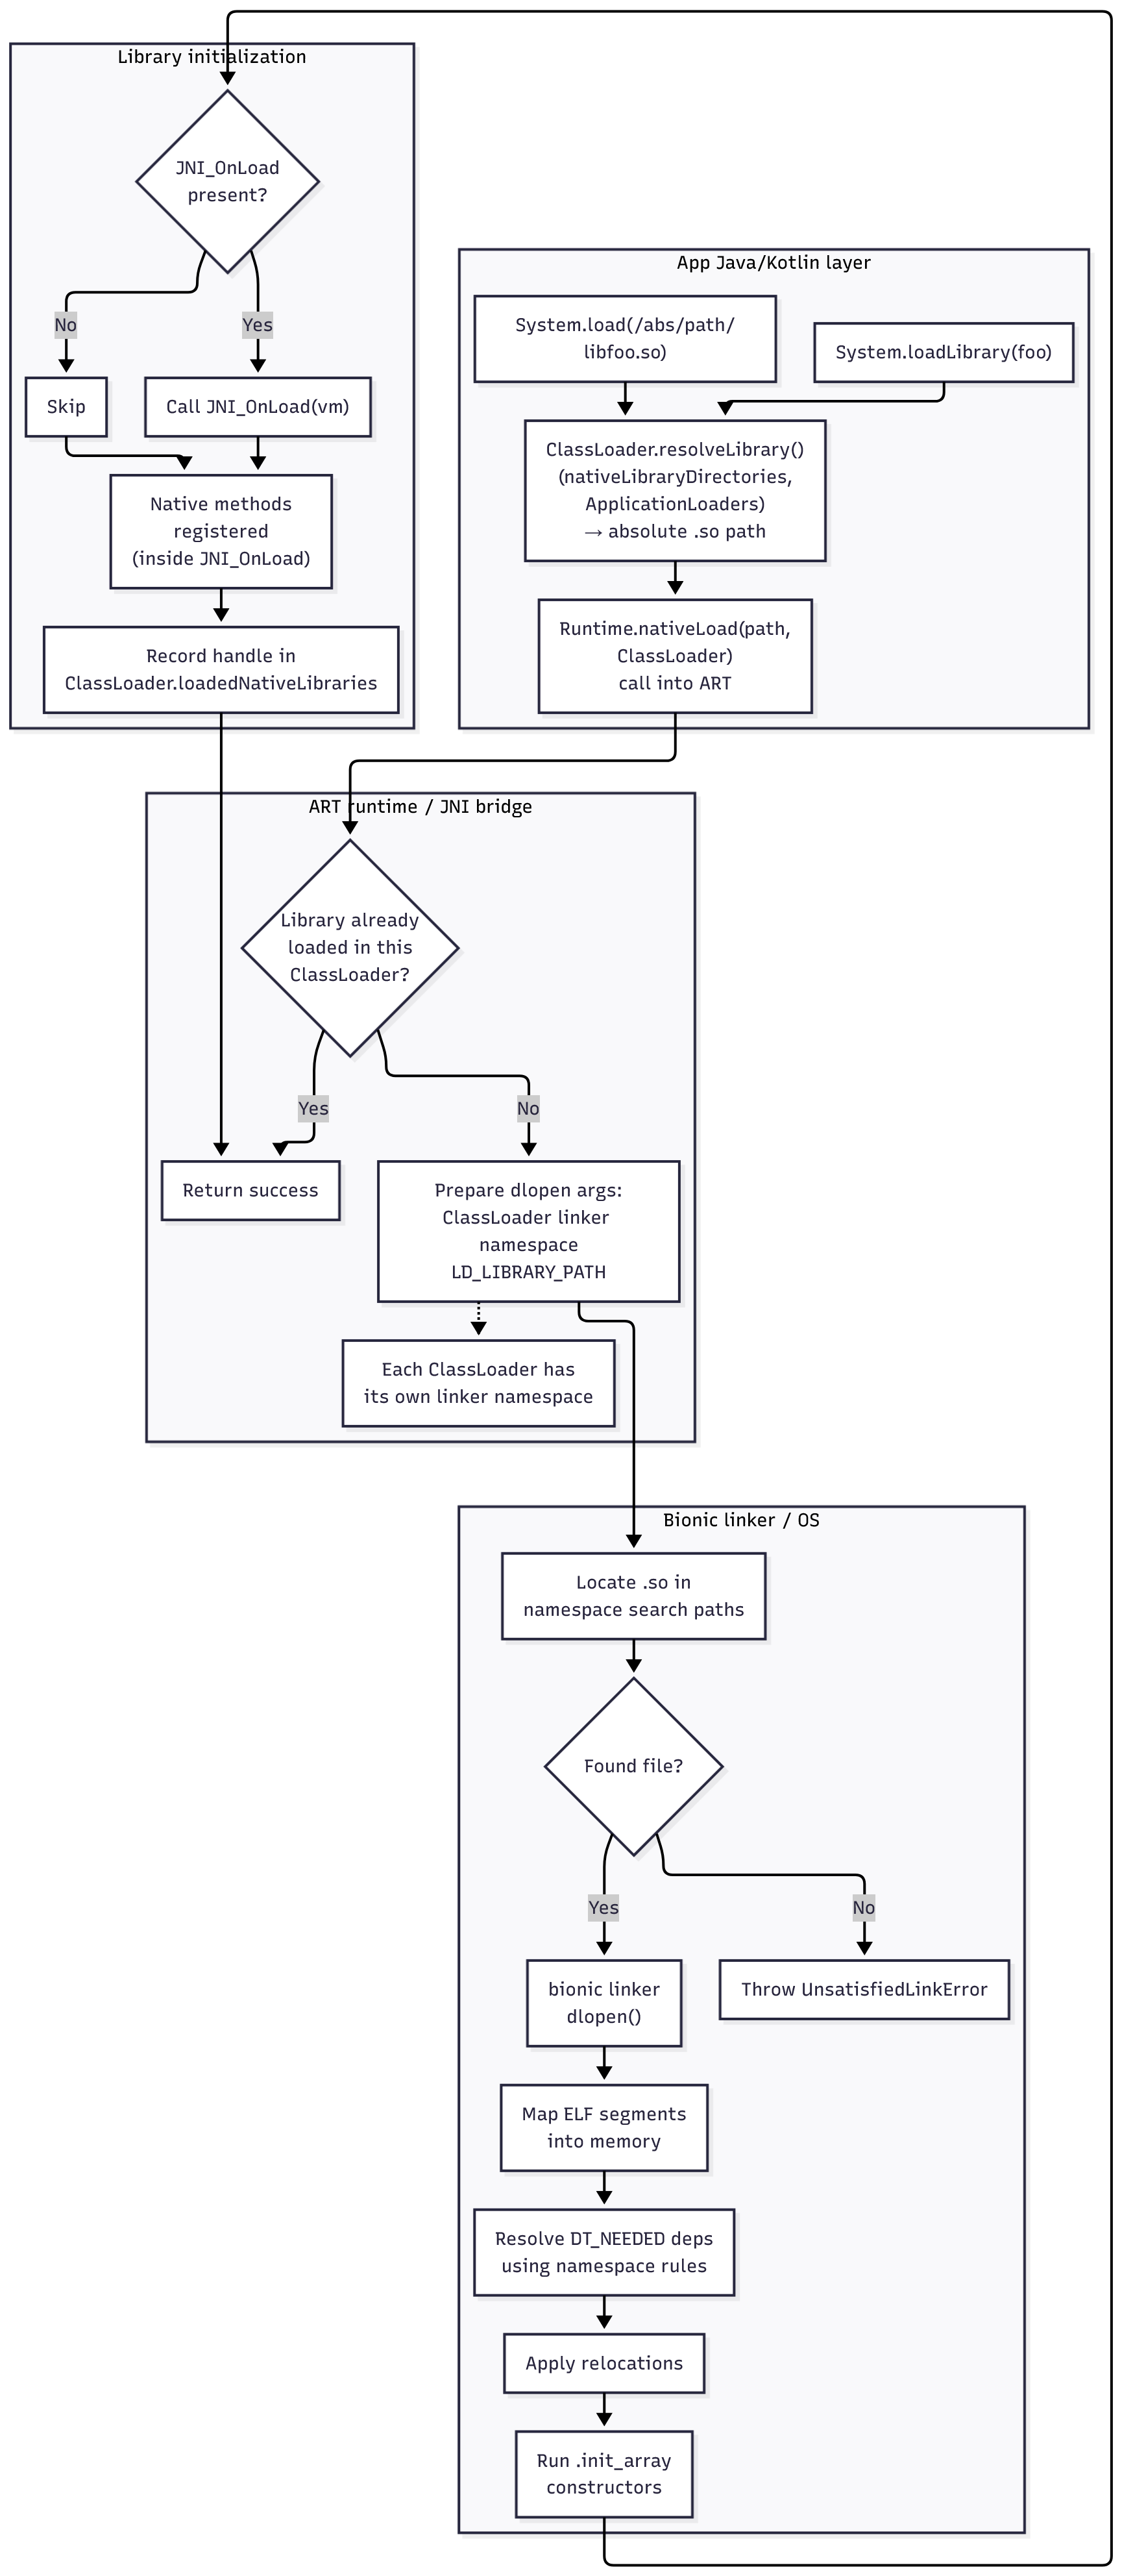
\includegraphics[width=0.65\textwidth]{images/android_application_native_library_loading_flow.png}
    \caption{Android application native library loading flow.}
    \label{fig:android_lib_load_flow}
\end{figure}

\subsection{Hooking and Interception Techniques}
\subsubsection{Java-level Hooking Methods}

Java-level hooking focuses on intercepting method calls at the managed code layer. It targets Android framework or application methods that execute in ART or a Java Virtual Machine (JVM)-like environment \cite{android_platform}.

One practical approach is method replacement through reflection. Using the \texttt{java.lang.reflect} API, private or system methods can be accessed, their accessibility modified, and their behavior overridden at runtime. This enables selective interception without repackaging the application.

Instrumentation frameworks such as Xposed~\cite{xposed2013framework} load a hook manager early in process startup and register handlers that run before or after targeted Java methods. In practice, a modified Zygote injects the Xposed bridge so modules can intercept framework and application APIs, substitute return values, and record arguments. Research systems extend this model to configurable monitors (e.g., Droidmon/ARTmon) that hook framework APIs and even mask environment fingerprints during analysis \cite{kumar2023inviseal}. Java-layer tools like Frida~\cite{frida2023official} can also attach to a running process and modify Java method behavior dynamically without prior application modification.

A key limitation of Java-level hooking is that it does not observe native-only execution. Java hooks cannot directly intercept native library loading through \texttt{dlopen()} or calls resolved purely in the dynamic linker. Anti-tamper checks may also detect injected managers or altered method paths, and modern policies constrain deployment on stock devices. Moreover, the compilation pipeline of ART (AOT/JIT) and the presence of native code in applications reinforce the boundary between managed and native execution, which motivates native-layer interception \cite{bleier2023oat,kumar2023inviseal,ronin2018hooking}.

\subsubsection{Native-level Hooking}

Native-level hooking intercepts compiled C/C++ execution and dynamic linking. It provides broader coverage, including system libraries and loader paths, at the cost of increased complexity \cite{ronin2018hooking}. In practice, native hooks can be implemented using several technique families, including inline patching of function prologues, PLT and Global Offset Table (GOT) based redirection, library interposition through load order control, and direct interception of loader entry points such as \texttt{dlopen()} and \texttt{dlsym()} \cite{ronin2018hooking,kumar2023inviseal}. The two techniques that are most relevant for this thesis, inline hooking and PLT-based hooking, are discussed in more detail in the following subsubsections.

\textbf{Library interposition.} This method replaces exported symbols by ensuring a custom library is loaded before the target. On Android, traditional \texttt{LD\_PRELOAD} is constrained by linker namespaces and application sandboxing. Effective interposition often relies on early injection, custom loader hooks, or process-specific load order control \cite{ronin2018hooking}. Research frameworks combine Java-layer hooks with operating system-level controls to reduce detectability while observing cross-layer behavior \cite{kumar2023inviseal}.

\textbf{Intercepting native loading.} Hooking \texttt{dlopen()} and related loader entry points allows observing, blocking, or replacing libraries as they map and relocate. This is essential when decrypting or unpacking protected libraries before use. Implementations must account for Android linker behavior, namespaces, and ART interactions \cite{ronin2018hooking,bleier2023oat}.

\textbf{Protections and detection.} Effective native hooks must handle Address Space Layout Randomization (ASLR), Security-Enhanced Linux (SELinux) constraints, and application integrity checks. Many applications verify code sections or loader state and may probe for modified tables or suspicious mappings. Analysis systems mitigate this by minimizing overhead, targeting hooks precisely, and correlating framework- and operating system-level signals \cite{kumar2023inviseal,ronin2018hooking}.

\subsubsection{Inline Hooking Techniques}

Inline hooking modifies instructions at the beginning of a function in order to redirect control flow to a custom handler before optionally returning to the original implementation. The typical pattern is to overwrite the function prologue with a branch instruction that jumps to a trampoline, which saves register state, executes custom logic, and then either calls the original function body or bypasses it completely. Because the overwritten instructions are lost when the branch is written, they must be relocated into the trampoline in a way that preserves original semantics, including correct handling of relative addresses and literal pools \cite{ronin2018hooking}.

On Android, inline hooks must account for the instruction set and calling conventions of the underlying CPU architecture. Historically, devices have used both ARM and Thumb instruction sets for 32 bit binaries, while modern devices predominantly use AArch64. Hooking frameworks therefore need to detect the current instruction mode, choose an appropriate branch encoding, and ensure that the trampoline is correctly aligned and resides in executable memory \cite{ronin2018hooking,kumar2023inviseal}. In environments with Address Space Layout Randomization (ASLR), the framework must compute target addresses at runtime rather than relying on fixed offsets.

Inline hooking has the advantage that it can target functions even when they are not exported through the dynamic symbol table. As long as the function address is known, either from static analysis or from in process symbol resolution, its prologue can be patched. This makes inline hooks suitable for intercepting internal helper functions or decryption routines that are deliberately hidden from the dynamic linker. At the same time, modifying code sections increases the risk of detection and instability, especially in applications that perform integrity checks on executable pages, verify code signatures, or rely on control flow integrity protections \cite{ronin2018hooking,kumar2023inviseal}. For these reasons, inline hooking is often combined with more conservative techniques such as PLT based redirection when observable behavior must remain as close as possible to the unmodified application.

\subsubsection{PLT-based Hooking Techniques}

PLT based hooking focuses on function calls that are resolved by the dynamic linker rather than patching instruction streams directly. In ELF based binaries, calls to external functions such as \texttt{dlopen()}, file I/O routines, or cryptographic APIs are compiled as indirect jumps through the Procedure Linkage Table. At runtime, the dynamic linker populates the corresponding entries in the Global Offset Table with the true target addresses. Once relocation is complete, every call through a PLT stub reads the function address from the GOT and branches to it. By modifying these GOT entries after they have been resolved, a hook can redirect all subsequent calls to a proxy implementation that executes custom logic before optionally delegating to the original function \cite{xinuos2025elf,ronin2018hooking}.

In contrast to inline patching, PLT based hooks operate entirely on data structures that the dynamic linker already manages. They do not require rewriting instructions in executable segments, which improves robustness across compiler optimizations and reduces the risk of violating code integrity checks. Hook implementations must still locate the relevant relocation entries, identify which GOT slots correspond to the targeted symbol, and update them atomically to avoid race conditions. Modern frameworks automate this process and also monitor newly loaded shared objects so that hooks are applied consistently as the set of loaded modules changes during execution \cite{ronin2018hooking,pizzi2022virtualpatch}.

For intercepting native library loading, PLT based techniques are particularly attractive. By targeting symbols such as \texttt{dlopen()} or \texttt{android\_dlopen\_ext()} in the process, a hook can observe every attempt to load a shared library, validate paths and flags, and transparently decrypt or unwrap protected binaries before forwarding the call. Because all callers of the symbol that resolve through the PLT share the same GOT entries, a single hook can cover multiple libraries and engine layers, which is beneficial in complex applications that embed several runtimes or plugin systems \cite{ronin2018hooking,pizzi2022virtualpatch}.

\subsection{Android Hooking Frameworks}

\subsubsection{Frida-based Hooking}

Frida is a dynamic instrumentation toolkit that allows developers, reverse engineers, and security researchers to observe and modify the behavior of applications at runtime on multiple platforms, including Android \cite{frida2023official}. In contrast to purely static patching, Frida injects a lightweight runtime into a live process and evaluates user supplied scripts that describe which functions to intercept and how to modify them. This model is well suited for exploratory analysis, rapid prototyping of hooks, and building custom monitoring tools without repackaging the target application.

On Android, Frida can operate in several configurations. On rooted devices, a \textit{frida-server} binary runs with sufficient privileges to attach to application processes and inject the Frida core. On non rooted devices, Frida can be embedded directly into an application or test harness through a special \textit{gadget} library that is loaded by the application. In both cases, the core component exposes an API to the external Frida client, which uploads and evaluates JavaScript based instrumentation logic inside the target process. This separation between transport and scripting makes it possible to iteratively refine hooks while the application is running \cite{frida2023official}.

Frida supports Java level instrumentation by interacting with the Android Runtime (ART). Scripts can enumerate loaded classes, access methods, and register handlers that execute before or after a selected Java method. For example, a script can intercept calls to \texttt{System.loadLibrary()} or to security related framework APIs, inspect arguments, modify return values, or short circuit a call entirely. Frida takes care of thread attachment, class loader resolution, and marshaling between Java types and script side objects, which lowers the barrier to building complex Java layer hooks compared to manual reflection based approaches \cite{frida2023official,kumar2023inviseal}.

In addition to Java methods, Frida exposes native level interception primitives that target compiled code in shared libraries. The most commonly used mechanism is attaching to a function address with an interceptor. A script can identify functions either by symbol name through module exports, such as \texttt{dlopen} or cryptographic routines, or by absolute address within a loaded module. Once attached, the hook receives callbacks on every function entry and exit, with access to register values and arguments. The script can then log or modify parameters, alter return values, or redirect control flow, which effectively implements inline hooks without manual patching of instruction bytes \cite{ronin2018hooking}.

Because Frida can observe both Java and native layers in the same process, it is particularly suitable for studying cross layer behavior such as native library loading. A typical pattern is to hook Java calls that request loading of a library and, in parallel, intercept the corresponding native \texttt{dlopen()} and \texttt{dlsym()} calls. This allows the analyst to correlate library names, file system paths, and resolved symbol addresses, and to verify when a protected library is mapped into memory. In scenarios where libraries are encrypted or unpacked at runtime, Frida scripts can target the decryption routines directly, dump decrypted code from memory, or delay execution until specific conditions are met \cite{ronin2018hooking,kumar2023inviseal}.

Despite its flexibility, Frida is primarily designed as an analysis and instrumentation tool rather than a production protection mechanism. The presence of the Frida core, its communication channels, and injected scripts can be detected by applications that perform integrity checks on process memory, open file descriptors, or loaded modules. Furthermore, Frida hooks are typically established from an external controller and are not persisted across application restarts without additional packaging. For the purposes of this thesis, Frida therefore serves mainly as a reference implementation and experimental platform for exploring hooking strategies, including the interception of native library loading paths, rather than as a direct candidate for integrating runtime decryption into production applications.

\subsubsection{LSPosed-based Hooking}

LSPosed is a modern implementation of the Xposed concept for recent Android versions. It is distributed as a Riru or Zygisk module and provides an Android Runtime (ART) hooking framework with APIs that remain compatible with the original Xposed framework \cite{xposed2013framework,lsposed2025github}. Internally, LSPosed leverages components such as LSPlant for ART level method interception and Dobby for inline hooking, while relying on systemless root solutions such as Magisk or KernelSU to inject its code into the \texttt{zygote} process \cite{lsposed2025github,lsposed2025website}. By doing so, it enables Java level hooks without modifying system partitions, which improves compatibility with over the air updates and reduces the risk of permanent system corruption compared to legacy, system modifying Xposed deployments \cite{androidroot2024lsposed,promon2024hooking}.

From an architectural perspective, LSPosed integrates into process startup at the point where the \texttt{zygote} forks new application processes. The LSPosed core is loaded into \texttt{zygote} via Magisk's Zygisk interface or Riru, so that every newly spawned app process inherits the framework. Xposed style modules are installed as regular Android applications and registered through the LSPosed manager. During app startup, LSPosed consults its configuration, loads the enabled modules, and invokes their callback entry points (such as \texttt{handleLoadPackage}) for the relevant packages. Modules then register hooks on selected Java methods in system or application code, using the familiar XposedBridge style API \cite{lsposed2025github,lsposed2025website,androidroot2024lsposed}.

\textit{Module scoping and configuration.} A central feature of LSPosed is fine grained scoping of modules. Instead of applying a module globally to the entire system, LSPosed lets the user restrict each module to specific applications, user profiles, or process types. This per app scoping reduces unintended side effects, simplifies troubleshooting, and improves security, because only the targeted processes are affected by a given hook \cite{androidroot2024lsposed,promon2024hooking}. LSPosed also integrates an online repository of modules, making it easier to discover and update functionality such as ad blocking, UI customization, or privacy enhancements directly from the manager interface \cite{lsposed2025website,androidroot2024lsposed}.

\textit{Platform coverage and limitations.} LSPosed is designed specifically for modern Android releases and supports versions from Android 8.1 up to Android 16 according to recent stable releases \cite{lsposed2025github,lsposed2025website,androidroot2024lsposed}. Because it operates as a systemless module in Magisk or KernelSU, it can typically persist across operating system updates as long as the underlying root solution remains compatible. At the same time, LSPosed is constrained to the managed layer: like the original Xposed, it hooks Java and Kotlin code running on ART and does not directly instrument native C/C++ code or the dynamic linker \cite{promon2024hooking}. Consequently, LSPosed can intercept high level calls such as \texttt{System.loadLibrary()} or security relevant framework APIs, but it cannot see native only library loading paths implemented purely with \texttt{dlopen()} and related functions in C/C++. For scenarios that require intercepting native library loading, observing ELF relocations, or decrypting libraries immediately before they are mapped, LSPosed is therefore complementary to, but not a replacement for, native level hooking techniques described elsewhere in this thesis.

\subsubsection{ByteHook-based PLT Hooking}

ByteHook is an open source Android PLT hook library developed by ByteDance. It provides a production-ready implementation of Procedure Linkage Table and Global Offset Table based hooking for native code, and is deployed in large scale applications such as TikTok, Douyin, Toutiao, Xigua Video, and Lark \cite{bytehook2025github}. In contrast to inline hook frameworks that modify instruction streams, ByteHook focuses on redirecting dynamically linked function calls by updating PLT and GOT entries at runtime. This approach aligns directly with the ELF-level linking model described earlier and avoids rewriting executable code sections, which improves portability and robustness across compiler optimizations and architectures \cite{pizzi2022virtualpatch}.

Architecturally, ByteHook targets functions that are imported from shared libraries and resolved through PLT stubs. For each hooked symbol, the library locates the corresponding GOT entries and replaces their contents with pointers to a proxy function. Subsequent calls that would normally reach the original function through the PLT instead invoke the proxy, which can inspect or modify arguments, perform additional logic, and optionally delegate to the original implementation \cite{bytehook2025github,pizzi2022virtualpatch}. ByteHook supports multiple independent hooks for the same symbol and can operate in three modes: it can hook a single caller library, a subset of caller libraries that match a filter, or all caller libraries in the process at once. It also monitors newly loaded dynamic libraries and applies hooks automatically to their PLT entries, which is essential when the set of loaded modules changes during execution \cite{bytehook2025github}.

Integration into an Android project is performed through a combination of Java and native components. ByteHook is distributed via Maven Central as an Android library that exposes a small Java API for initialization. During application startup, a call such as \texttt{ByteHook.init()} configures the global hooking environment inside the process \cite{bytehook2025github,bytehook2025maven}. Native modules then link against the provided \texttt{libbytehook.so} using CMake or \texttt{Android.mk} build scripts and invoke the C API (for example, \texttt{bytehook\_hook\_single}, \texttt{bytehook\_hook\_partial}, or \texttt{bytehook\_hook\_all}) to register hooks on specific symbols. Each hook is represented by a stub handle that can later be used to remove the hook or query its state. Helper macros manage per-thread hook stacks and ensure that calls back into the original function do not introduce recursion or inconsistent nesting \cite{bytehook2025github}.

ByteHook is relevant as a practical mechanism for intercepting native library loading and other critical runtime functions without modifying the operating system or requiring root privileges. By targeting symbols such as \texttt{dlopen()}, \texttt{android\_dlopen\_ext()}, or other loader related entry points in the appropriate shared libraries, ByteHook can observe and redirect native loading operations at the PLT level. A proxy function can validate requested paths, enforce policy, or transparently decrypt protected libraries before forwarding the call to the original loader routine. Because ByteHook is capable of hooking all callers of a given symbol across all dynamic libraries and automatically tracking newly loaded modules, it can provide comprehensive coverage for native loading flows in complex applications that rely on multiple runtime environments and engine style code \cite{bytehook2025github,pizzi2022virtualpatch}.

\subsection{Summary of relevant technologies}

This section has outlined the key technical foundations required for the proposed protection system. The Android platform was introduced as a layered software stack built on a modified Linux kernel, with native libraries packaged as ELF shared objects and exposed to applications through the Android Runtime (ART) and the Java Native Interface (JNI). The discussion of ELF structure, dynamic symbol resolution, and library loading mechanisms highlighted how the dynamic linker maps \texttt{.so} files into memory, resolves dependencies via PLT and GOT entries, and enforces class loader and namespace boundaries during \texttt{System.loadLibrary()} and \texttt{dlopen()} calls.

Hooking and interception techniques were then surveyed at both the Java and native layers. Java-level methods, including reflection-based interception and ART focused frameworks such as Xposed and LSPosed, provide powerful instrumentation of managed code but cannot observe purely native loading paths or low level linker behaviour. Native-level techniques, in particular inline hooks and PLT based hooks, extend coverage to compiled C/C++ code and dynamic linking, enabling interception of functions such as \texttt{dlopen()} and \texttt{android\_dlopen\_ext()} at the point where libraries are actually mapped and initialised.

Finally, representative Android hooking frameworks were reviewed. Frida illustrates a flexible, script driven approach that spans both Java and native layers and is well suited for analysis and prototyping. LSPosed demonstrates a modern, systemless evolution of Xposed that focuses on ART level method interception. ByteHook provides a production oriented implementation of PLT based hooking that operates entirely within native code and is already deployed in large scale applications. Together, these technologies motivate and enable the proof of concept system developed in this thesis, which relies on PLT based interception of native loading calls to decrypt and load protected libraries at runtime without modifying the Android platform.

\newpage

\section{System specification}
\label{sec:spec}

\subsection{System purpose and scope}

The system developed in this thesis is a proof of concept runtime protection mechanism for Android applications that rely on native libraries. Its primary purpose is to ensure that selected native libraries are stored on disk only in encrypted form and are decrypted solely inside the application process at runtime, immediately before being loaded by the Android dynamic linker. The system targets scenarios where native libraries are loaded not only from Java or Kotlin code but also from other native libraries, so that nested native to native loading flows are covered in the same way as direct loads.

The system consists of two main parts. The first part is a build time encryption component integrated into the Android project build pipeline. This component processes compiled shared objects and replaces selected libraries with encrypted equivalents that are no longer valid ELF binaries from the operating system point of view. The resulting encrypted libraries are packaged into the APK in the standard locations for native code so that the Android installation and extraction process remains unchanged.

The second part is a runtime protection component embedded into the protected application. This component initializes a native hooking mechanism during application startup and intercepts all calls to the native library loading functions in the current process, regardless of their origin. The component maintains a registry of protected library names and routes every intercepted loading request through a proxy function that performs a lookup against this registry. When the requested library is found in the protected list, the proxy locates the corresponding encrypted file on disk, decrypts its contents in memory, and loads the decrypted image into the process using an in memory file descriptor. For libraries that are not in the protected list, the proxy forwards the loading request directly to the original dynamic linker implementation without modification. This design preserves normal application behavior for unprotected components while selectively applying decryption only where needed.

The scope of the system is limited to in process protection for a single Android application. The design assumes that the application can be rebuilt in order to add the build time encryption step and to link against the native protection library. The system does not attempt to provide system wide protection, cross process enforcement, or integration with hardware backed key storage. It also does not implement anti debugging or anti hooking countermeasures. Instead, the goal is to demonstrate that transparent decryption and loading of protected native libraries is feasible on stock Android devices under realistic deployment constraints.

The high level scope and placement of the system within the Android execution environment are summarized in \cref{fig:system_scope_mermaid}.

\begin{figure}[p]
    \centering
    \includesvg[width=1\textwidth]{images/high_level_overview_of_proposed_system.svg}
    \caption{High level overview of the proposed protection system.}
    \label{fig:system_scope_mermaid}
\end{figure}

\subsection{Operating environment and assumptions}

The proposed system is designed and evaluated as an in process protection mechanism for a single Android application running on stock devices without root. It does not modify the operating system, the Android Runtime (ART), or the system linker, and relies only on APIs and behaviors available to a regular application process.

The minimum platform level for which this proof of concept is specified is Android 8.0 (API level 26). This lower bound is determined by the combined requirements of the native loading and in memory execution mechanisms. The system relies on the Android specific \texttt{android\_dlopen\_ext} function with the \texttt{ANDROID\_DLEXT\_USE\_LIBRARY\_FD} flag to load decrypted libraries from a file descriptor \cite{android_ndk_dlext}, and on the \texttt{memfd\_create} syscall to obtain an anonymous in memory file. The \texttt{android\_dlopen\_ext} function with the \texttt{ANDROID\_DLEXT\_USE\_LIBRARY\_FD} flag is officially available from API level 21. The \texttt{memfd\_create} functionality is invoked directly as a raw Linux syscall via \texttt{syscall(\_\_NR\_memfd\_create, \ldots)}, bypassing the C library wrapper entirely. This syscall was introduced in Linux kernel 3.17, which is present on all devices shipping with Android 8.0 or higher. Because the implementation does not rely on the C library \texttt{memfd\_create} wrapper (which was only added in API level 30), the effective minimum is Android 8.0 (API level 26).

The system targets ARM based devices and is built for the \texttt{armeabi-v7a} and \texttt{arm64-v8a} application binary interfaces. In practice, the implementation and evaluation focus on 64 bit devices using the \texttt{arm64-v8a} ABI, while 32 bit support is treated as best effort rather than a primary objective. No x86 or x86\_64 builds are included in the current prototype.

From the application perspective, the system is implemented as a proof of concept within a dedicated demo application that bundles both the protection library and the protected native libraries. The long term goal is to provide the protection logic as a reusable native library that third party developers could link into their own applications and configure for their specific set of protected libraries. For the purposes of this thesis, the deployment model is restricted to a single application that can be rebuilt as needed to integrate the build time encryption step and the runtime protection component.

The build and development toolchain used for the system consists of Android Studio with Gradle for project management, the Android NDK with CMake for compiling native C/C++ code, and Python for implementing the proof of concept encryption tool that processes compiled shared objects during the build. The design assumes that the application is packaged in the standard way for native libraries and that the manifest is configured with \texttt{android:extractNativeLibs="true"} so that the operating system extracts shared libraries to the application specific \texttt{/data/app/.../lib/<abi>/} directory. This extraction behaviour is relied upon to locate the encrypted library files on disk at runtime.

In summary, the system specification assumes an unmodified Android 8.0 (API level 26) or newer environment, ARM based application binaries, a rebuildable application under the control of the developer, and a modern Android toolchain with both native and scripting capabilities. Any behaviour outside these bounds, such as legacy devices with older kernels or custom system images with different linker behaviour, is considered out of scope for this proof of concept.

\subsection{System requirements}

This subsection defines the main functional and non functional requirements for the proposed protection system. Security related requirements are included as part of the non functional requirements.

\subsubsection{Functional requirements}

\begin{table}[H]
    \centering
    \caption{Functional requirements}
    \label{tab:functional_requirements}
    \begin{tabular}{|p{0.06\textwidth}|p{0.14\textwidth}|p{0.20\textwidth}|p{0.49\textwidth}|}
        \hline
        \textbf{ID} & \textbf{Type} & \textbf{Name} & \textbf{Description} \\
        \hline
        FR1 & Build time &
        Build time encryption of selected libraries &
        Selected native shared libraries shall be encrypted after compilation and their encrypted versions shall replace the original \texttt{.so} files before packaging. \\
        \hline
        FR2 & Packaging &
        Preservation of standard packaging and installation &
        Encrypted libraries shall be placed in the standard native library locations inside the APK so that Android packaging, installation, and extraction behaviour are unchanged. \\
        \hline
        FR3 & Initialization &
        Runtime initialization of the protection component &
        The runtime protection component shall be initialized during application startup before any protected library is loaded. \\
        \hline
        FR4 & Interception &
        Interception of native library loading calls &
        The system shall intercept native library loading calls in the protected process, regardless of whether they originate from managed code or other native libraries. \\
        \hline
        FR5 & Routing &
        Registry driven routing of load requests &
        The system shall maintain a registry of protected library identifiers and shall route each intercepted load request through either the decryption path or the normal loading path based on this registry. \\
        \hline
        FR6 & Loading &
        Decryption and loading of protected libraries &
        For libraries marked as protected, the system shall locate the encrypted file on disk, decrypt it in memory, and load the resulting shared object into the current process using an in memory file descriptor or equivalent mechanism. \\
        \hline
        FR7 & Compatibility &
        Transparent loading of unprotected libraries &
        For libraries that are not marked as protected, the system shall forward load requests directly to the original dynamic linker implementation without changing their behaviour. \\
        \hline
        FR8 & Compatibility &
        Support for nested native to native loading &
        The system shall apply interception and routing decisions to native library loads that are initiated from already loaded native libraries in the same process. \\
        \hline
        FR9 & Robustness &
        Error reporting and failure handling &
        On failure to decrypt or load a protected library, the system shall report the error through diagnostics and return a failure to the caller, without executing partially decrypted or invalid code. \\
        \hline
    \end{tabular}
\end{table}

\subsubsection{Non functional requirements}

\begin{table}[H]
    \centering
    \caption{Non functional requirements}
    \label{tab:nonfunctional_requirements}
    \begin{tabular}{|p{0.06\textwidth}|p{0.14\textwidth}|p{0.20\textwidth}|p{0.49\textwidth}|}
        \hline
        \textbf{ID} & \textbf{Type} & \textbf{Name} & \textbf{Description} \\
        \hline
        NFR1 & Performance &
        Startup overhead &
        Initialization of the protection component and hook installation shall not introduce excessive cold start overhead on a representative test device. \\
        \hline
        NFR2 & Performance &
        Overhead for unprotected libraries &
        Additional overhead for loading libraries that are not protected shall be minimal compared to a direct call to the dynamic linker. \\
        \hline
        NFR3 & Reproducibility &
        Build reproducibility &
        With the same source code and configuration, the build process including the encryption step shall produce consistent outputs. \\
        \hline
        NFR4 & Maintainability &
        Maintainability and configurability &
        Adding or removing protected libraries shall require changes only in a limited set of configuration points, such as the protection registry and build settings. \\
        \hline
        NFR5 & Compatibility &
        Toolchain compatibility &
        The system shall integrate into an Android Studio, Gradle, NDK, and CMake based toolchain without modifications to platform tools or system components. \\
        \hline
        SR1 & Confidentiality &
        No valid protected libraries on disk &
        In the installed application, protected libraries shall not exist on disk as valid loadable shared objects and their encrypted replacements shall not be accepted directly by the dynamic linker. \\
        \hline
        SR2 & Confidentiality &
        Decryption confined to process memory &
        Decryption of protected libraries shall occur only in the memory of the protected process and decrypted content shall not be written to persistent storage. \\
        \hline
        SR3 & Confidentiality &
        Controlled lifetime of decrypted content &
        Decrypted content shall be retained only as needed to map the library into the process and no additional plaintext copies shall be kept beyond what is required for execution. \\
        \hline
        SR4 & Fail safe &
        Fail safe behaviour on errors &
        If decryption or loading of a protected library fails, the system shall not load the library and shall not fall back to any plaintext version of the same library. \\
        \hline
        SR5 & Cryptographic agility &
        Algorithm agnostic design &
        The interception, routing, and in memory loading logic shall be designed to allow replacement of the encryption algorithm and key management approach without redesigning the core interception, routing, and loading mechanism. \\
        \hline
    \end{tabular}
\end{table}

\subsection{Summary of the system specification}

In summary, the specified system pairs a build-time encryption step with a runtime interception component.  At build time, a post-build script XOR-encrypts chosen \texttt{.so} files in place, producing invalid ELF binaries that ship inside the APK at the standard native library locations.  At runtime, a PLT-based hook on \texttt{\_\_loader\_dlopen} intercepts every native library load, consults a registry of protected filenames, and either forwards unprotected requests to the original loader or diverts protected ones through an in-memory decrypt-validate-load path backed by \texttt{memfd\_create} and \texttt{android\_dlopen\_ext()}.

The target platform is ARM-based Android 8.0+ (API~26) with an unmodified stock OS, a rebuildable application, and the \texttt{android:extractNativeLibs="true"} manifest flag.  Functional requirements cover build-time encryption validity, transparent interception of nested native-to-native loads, and strict fail-safe behaviour.  Non-functional requirements bound startup overhead and mandate reproducible builds.  Security requirements stipulate that no plaintext protected library may exist on persistent storage, that decrypted content must remain confined to process memory, and that the interception logic must be independent of any specific cipher so that cryptographic strength can be upgraded without redesigning the loading pipeline.

\newpage

\section{System implementation}

\subsection{System architecture}

This subsection maps out the proof-of-concept structure and explains why responsibilities are split the way they are.  Two distinct stages exist: a build-time stage that invalidates selected libraries on disk, and a runtime stage that restores them exclusively in process memory.

\subsubsection{Component responsibilities}

Six logical components make up the system.

\begin{itemize}
    \item \textbf{Build-time encryption tool (Python).}
    A post-build step that XOR-encrypts selected compiled \texttt{.so} files in place.  The resulting file replaces the original so the APK ships only the encrypted variant.  Details appear in the \textit{Build-time encryption implementation} subsection.

    \item \textbf{Java bootstrap for load order.}
    The \texttt{NativeCallHook} class, whose sole architectural role is to guarantee that the protection library is mapped and its constructor executed before any other native library is loaded.  See \textit{Java-Native integration and load order}.

    \item \textbf{Native protection library (\texttt{libnativecallhook.so}).}
    Contains the hook-installation constructor and the interception callback.  See \textit{Runtime hook initialization}.

    \item \textbf{Hooking framework (ByteHook).}
    A third-party PLT/GOT interception library.  It patches GOT entries process-wide and propagates patches to libraries loaded after hook installation.

    \item \textbf{Protected library registry and routing logic.}
    A compile-time list of filenames consulted inside the hook callback to decide between normal loading and the decryption path.  See \textit{Protected library registry and routing logic}.

    \item \textbf{In-memory decryption and loader handoff.}
    Reads encrypted bytes from disk, XOR-decrypts them, validates the ELF header, writes the plaintext to an anonymous \texttt{memfd} descriptor, and hands it to the Android linker.  See \textit{In-memory decryption and loading}.
\end{itemize}

\cref{fig:component_diagram} shows how these components relate across the build-time / runtime boundary.  \cref{fig:class_diagram} maps them to concrete source files, classes, and their dependencies.

\begin{figure}[p]
    \centering
    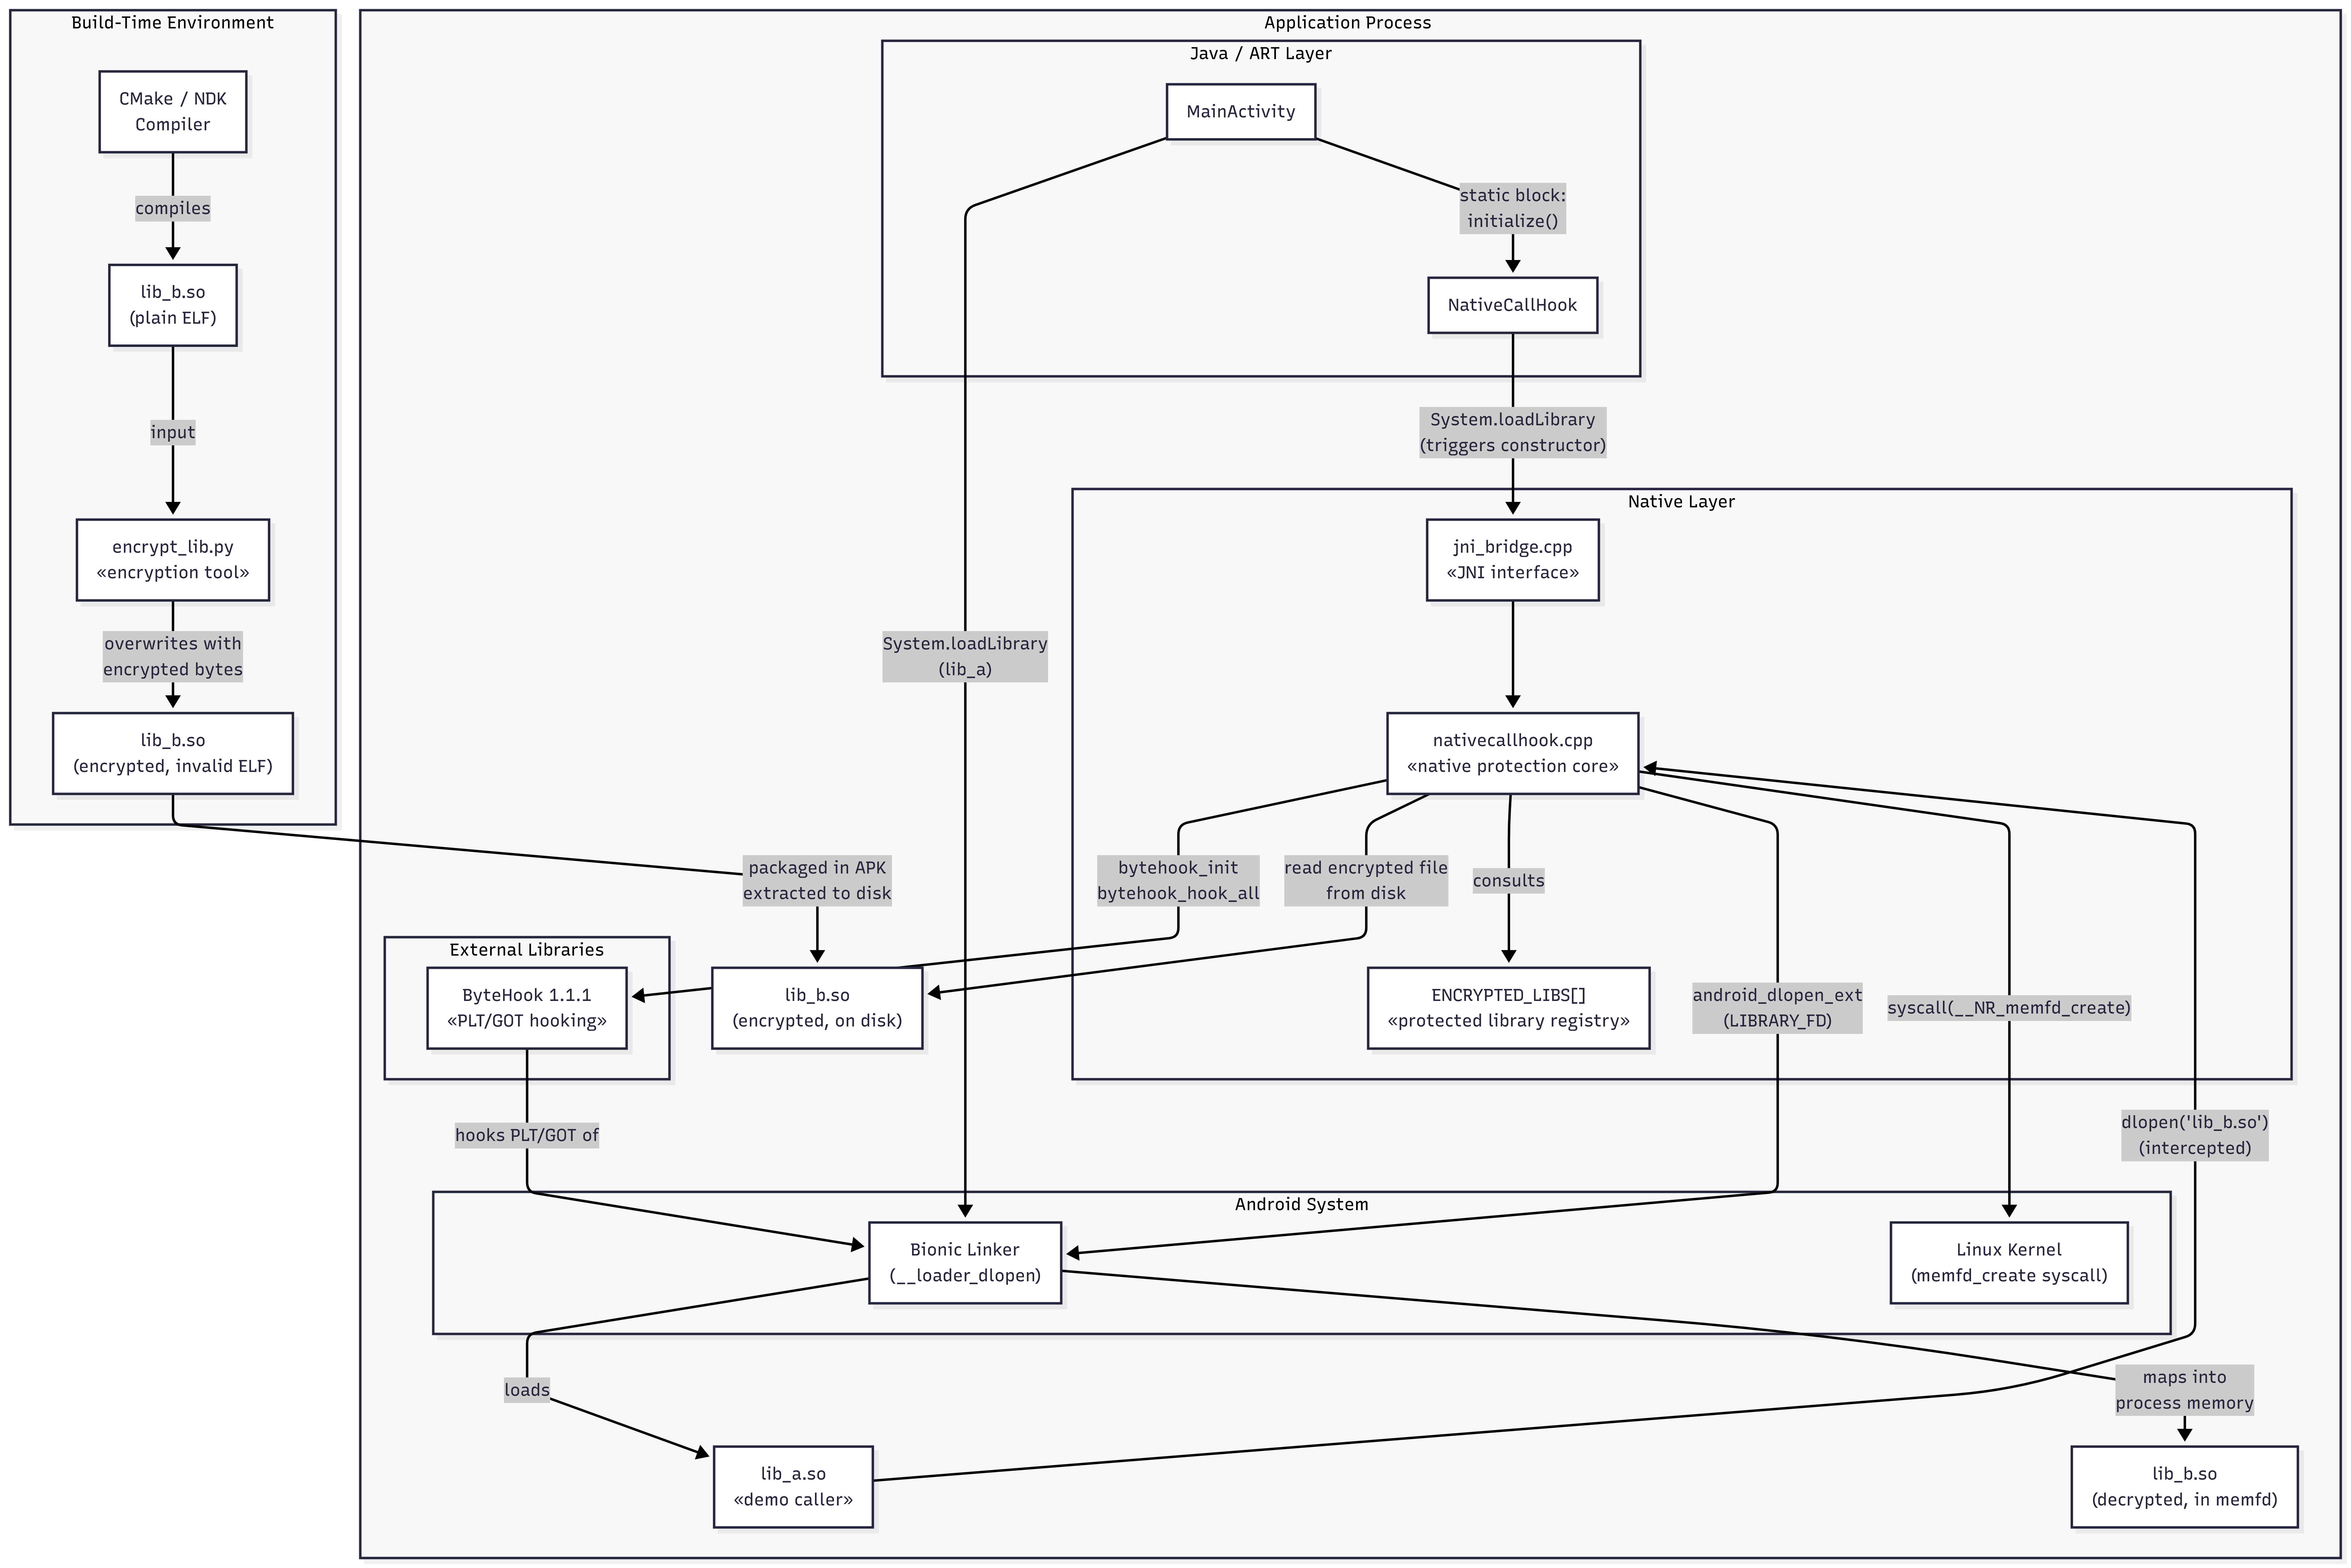
\includegraphics[width=0.7\textwidth]{images/component.png}
    \caption{Component diagram of the protection system.}
    \label{fig:component_diagram}
\end{figure}

\begin{figure}[p]
    \centering
    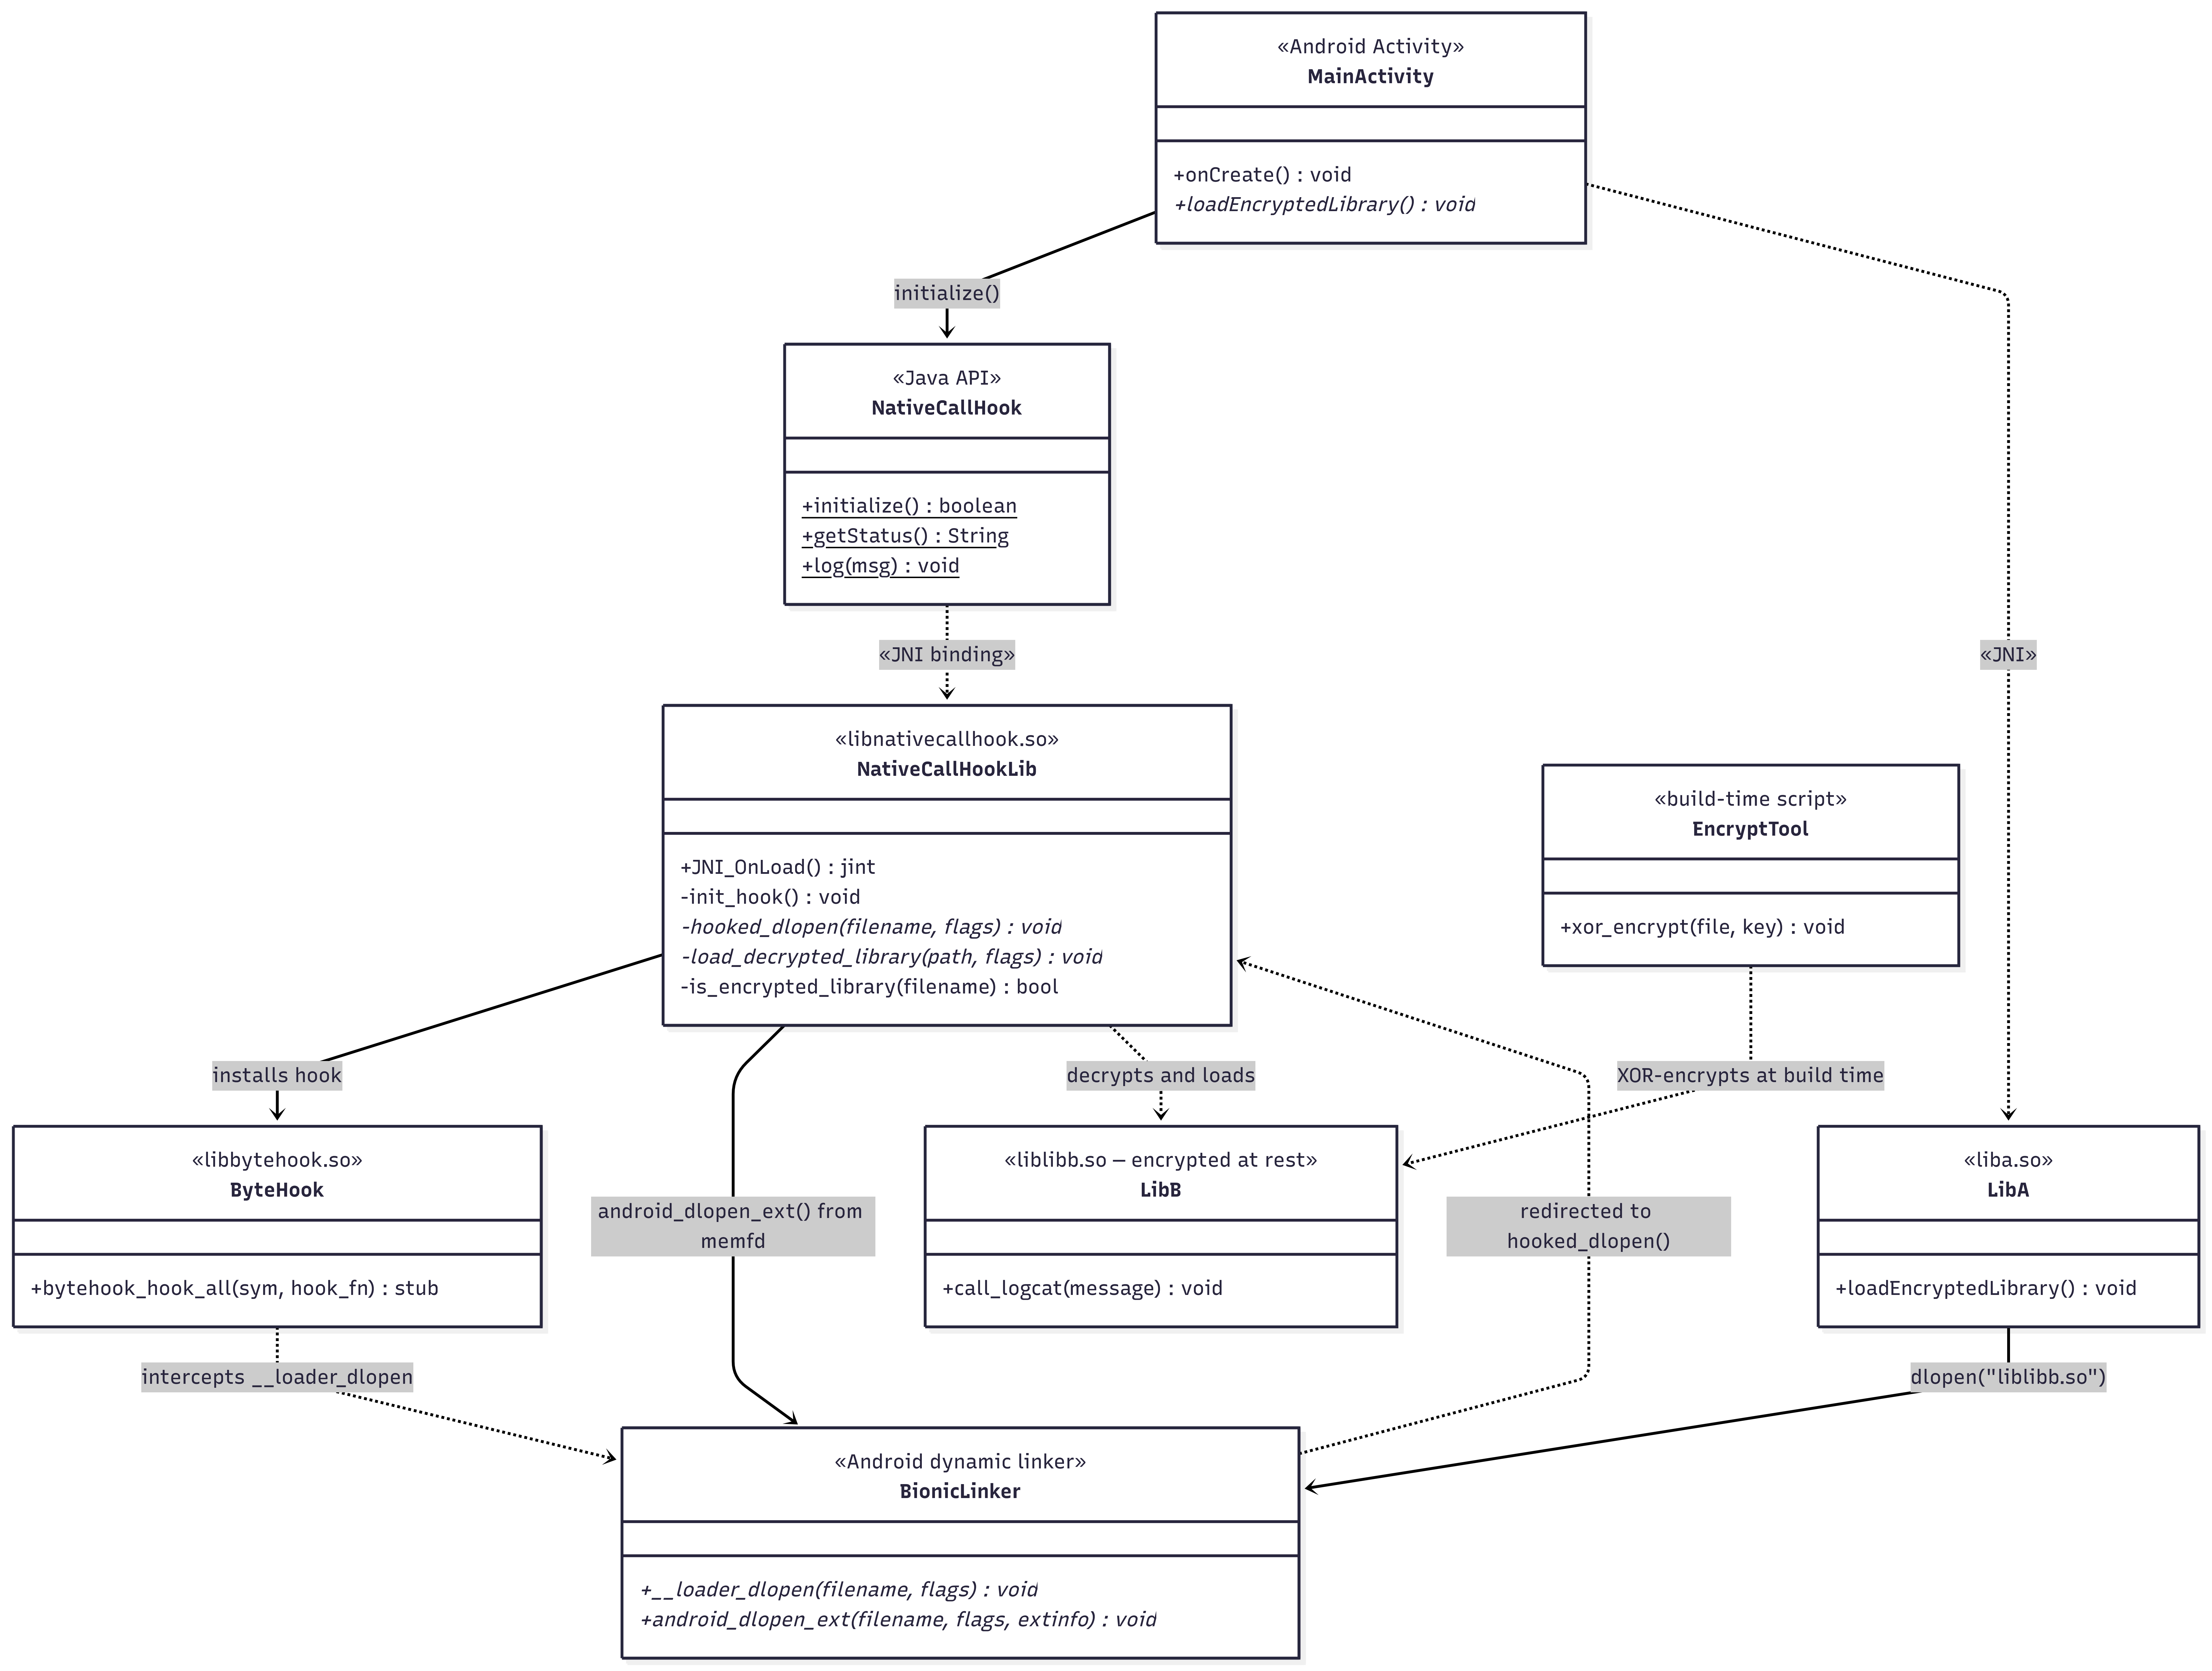
\includegraphics[width=1\textwidth]{images/class_diagram.png}
    \caption{Class diagram of the protection system, showing the relationships between Java and native modules.}
    \label{fig:class_diagram}
\end{figure}

\subsubsection{End-to-end execution flow}

The pipeline spans both stages:

\begin{enumerate}
    \item \textbf{Build-time transformation.}
    The NDK toolchain compiles native libraries normally.  Afterwards, the encryption script overwrites the target library (\texttt{liblibb.so}, labelled \texttt{lib\_b.so} in diagrams) with its XOR-encrypted form, destroying the ELF header and rendering the file unloadable by the default linker.

    \item \textbf{Process startup and hook activation.}
    The Java bootstrap loads \texttt{libnativecallhook.so} early.  Its ELF constructor installs the PLT hook during the \texttt{System.loadLibrary()} call, before control returns to the JVM.

    \item \textbf{Interception boundary.}
    The constructor patches \texttt{\_\_loader\_dlopen} process-wide, which is the internal symbol through which both managed-to-native and native-to-native \texttt{dlopen}-family calls eventually pass.

    \item \textbf{Per-request routing.}
    Each intercepted call is checked against the registry.  Unmatched requests are forwarded to the original loader with no modification.

    \item \textbf{Decrypt-and-load for protected libraries.}
    Matched requests trigger file read, XOR decryption, ELF-header validation, \texttt{memfd\_create} + \texttt{write()}, and finally \texttt{android\_dlopen\_ext()} with \texttt{ANDROID\_DLEXT\_USE\_LIBRARY\_FD}.  No plaintext reaches disk.

    \item \textbf{Nested loading coverage.}
    Because the hook is process-wide, a native library that itself calls \texttt{dlopen()} for another protected library follows the identical decrypt-and-load path, which is precisely the scenario that motivates this thesis.
\end{enumerate}

The interaction between components during hook installation and a protected library load is shown in \cref{fig:sequence_diagram}.

\begin{figure}[p]
    \centering
    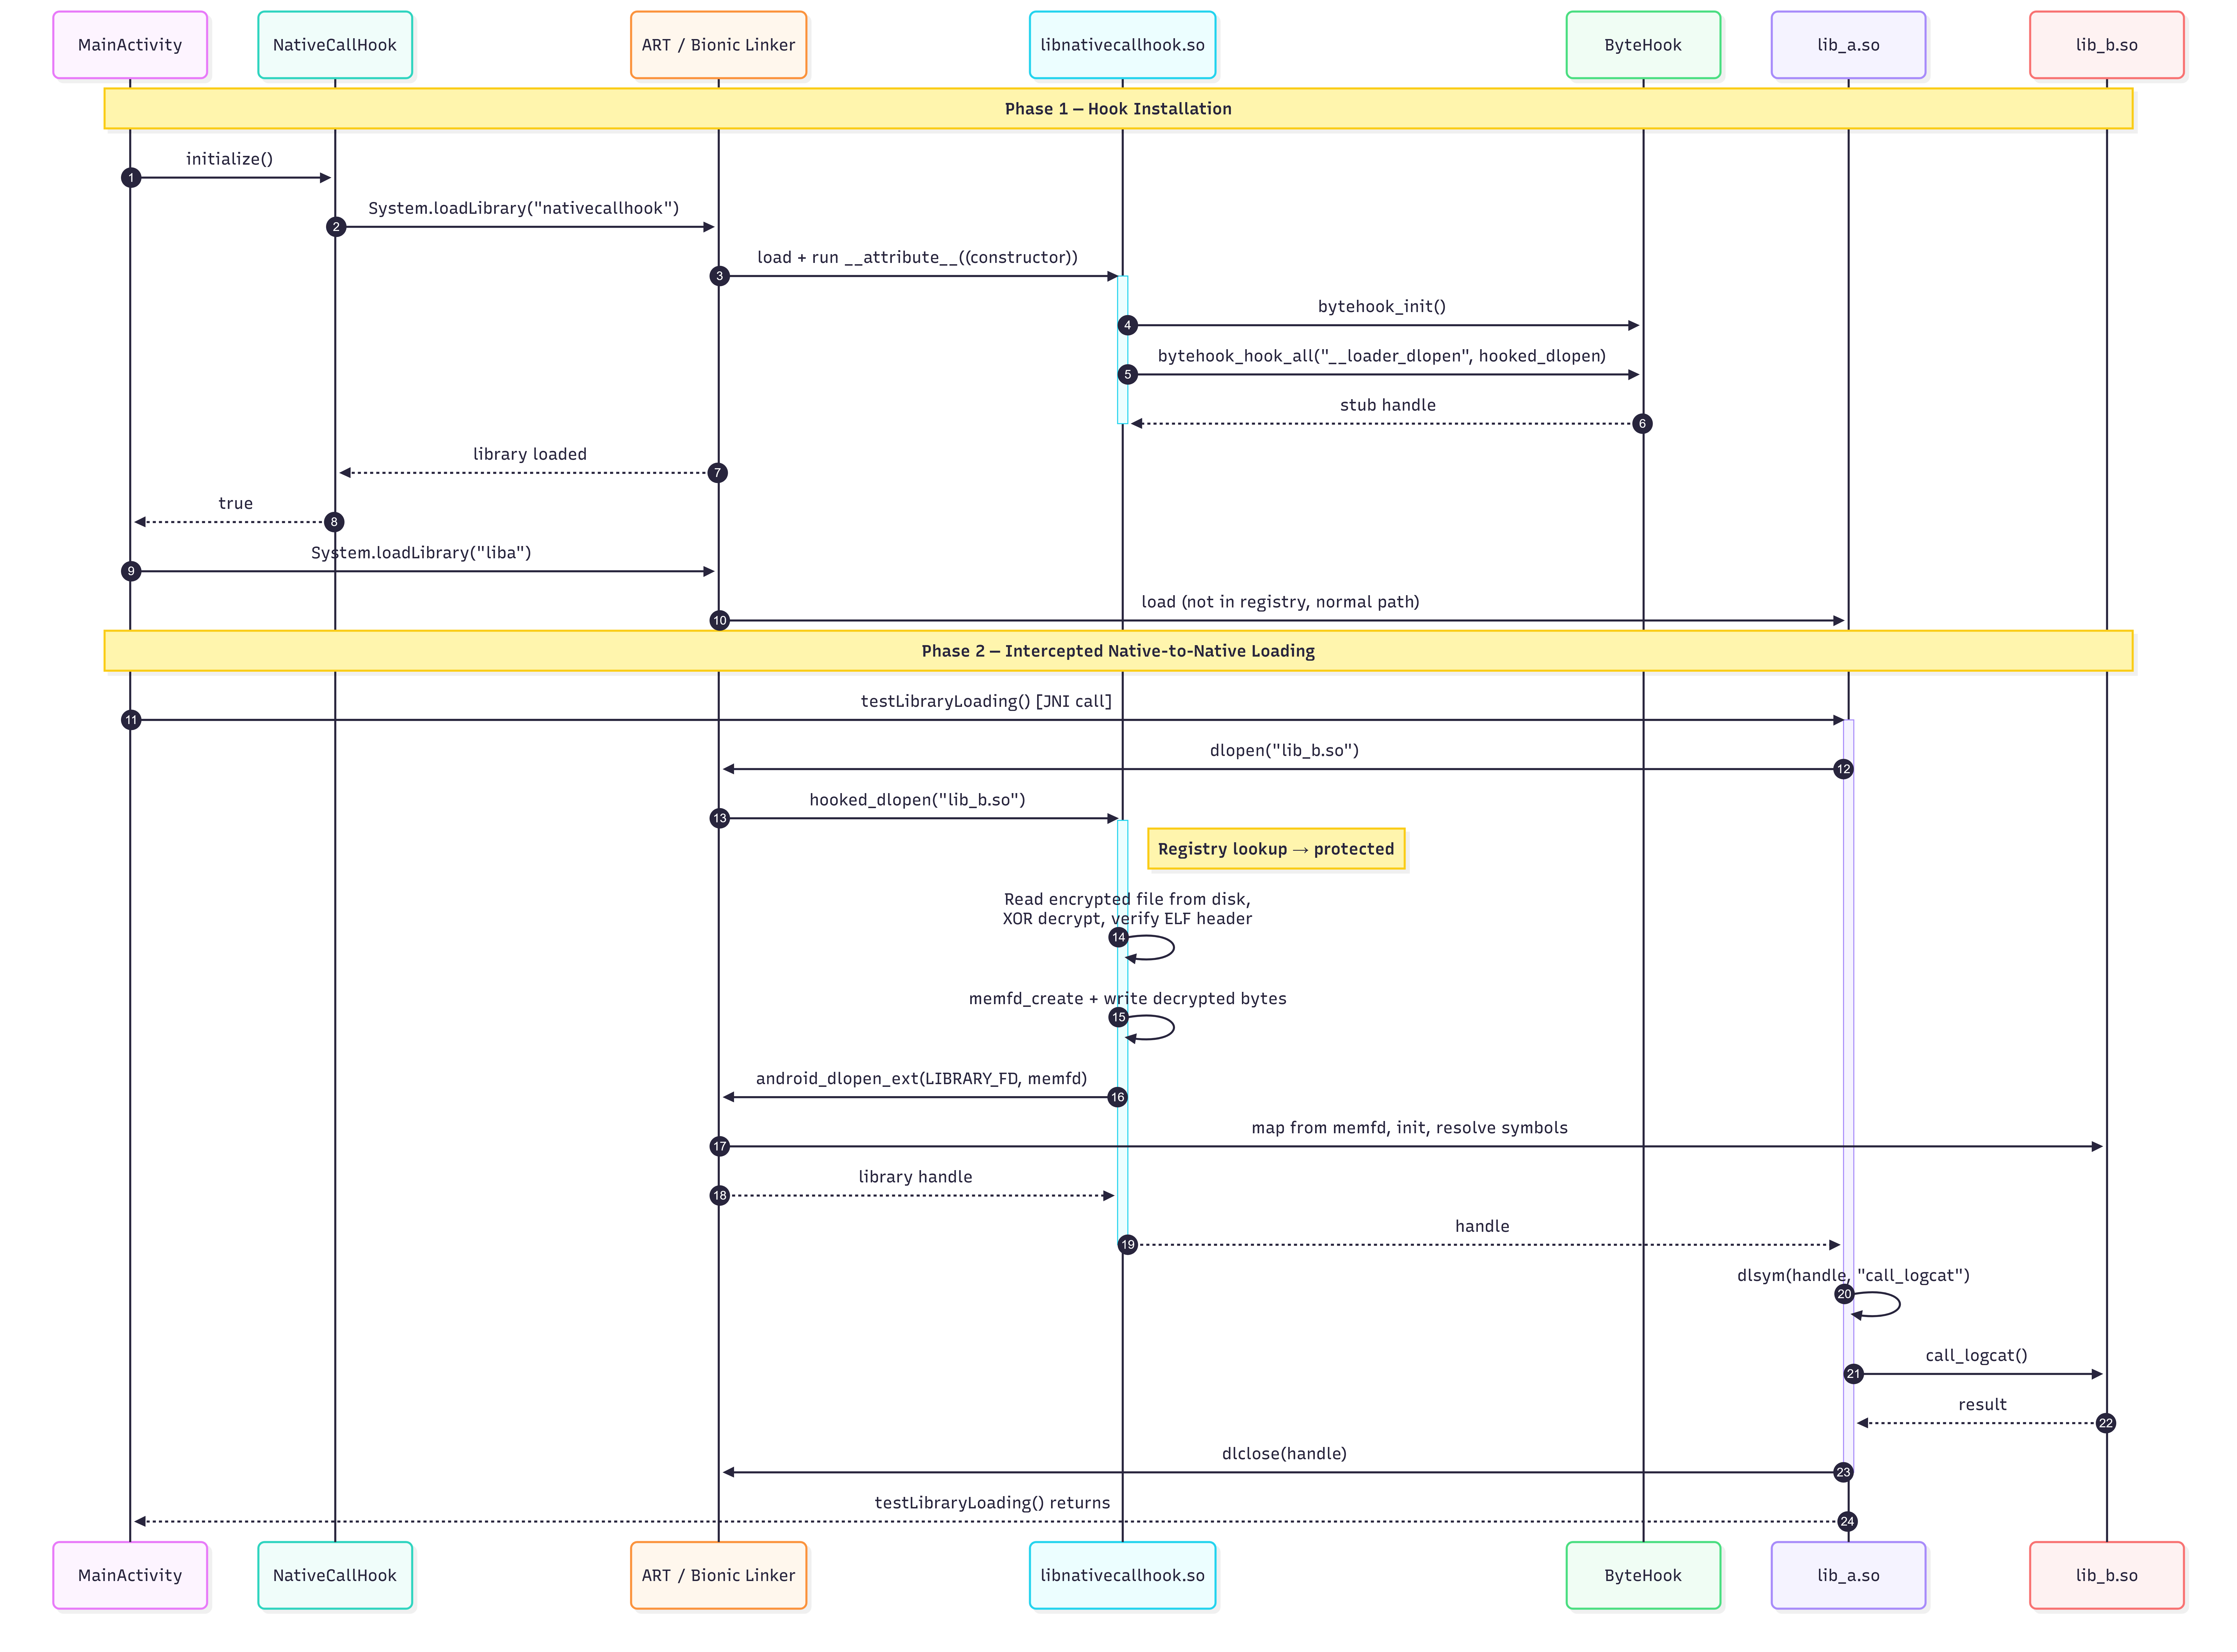
\includegraphics[width=1\textwidth]{images/sequence.png}
    \caption{Sequence diagram of hook installation and encrypted library loading.}
    \label{fig:sequence_diagram}
\end{figure}

\subsubsection{Architectural assumptions and scope boundaries}

The architecture relies on two explicit assumptions that directly shape the implementation.
\begin{itemize}
    \item \textbf{Standard native library extraction is enabled.} The routing and path-resolution logic assumes that the application libraries exist on disk in the usual extracted directory (for example when \texttt{android:extractNativeLibs="true"} is used), so the encrypted library can be located and read as a file before decryption.
    \item \textbf{Proof-of-concept cryptography and configuration.} The encryption key and the protected-library list are intentionally static in this prototype. This choice simplifies the architecture so the thesis can focus on the interception, routing, and in-memory loading mechanism rather than production-grade key management.
\end{itemize}

The physical distribution of artifacts across the developer machine, the APK, and the target device is shown in \cref{fig:deployment_diagram}. The diagram highlights that the encrypted library exists as an invalid ELF on persistent storage and is only restored to a loadable state inside process memory through the memfd-backed decryption path.

\begin{figure}[p]
    \centering
    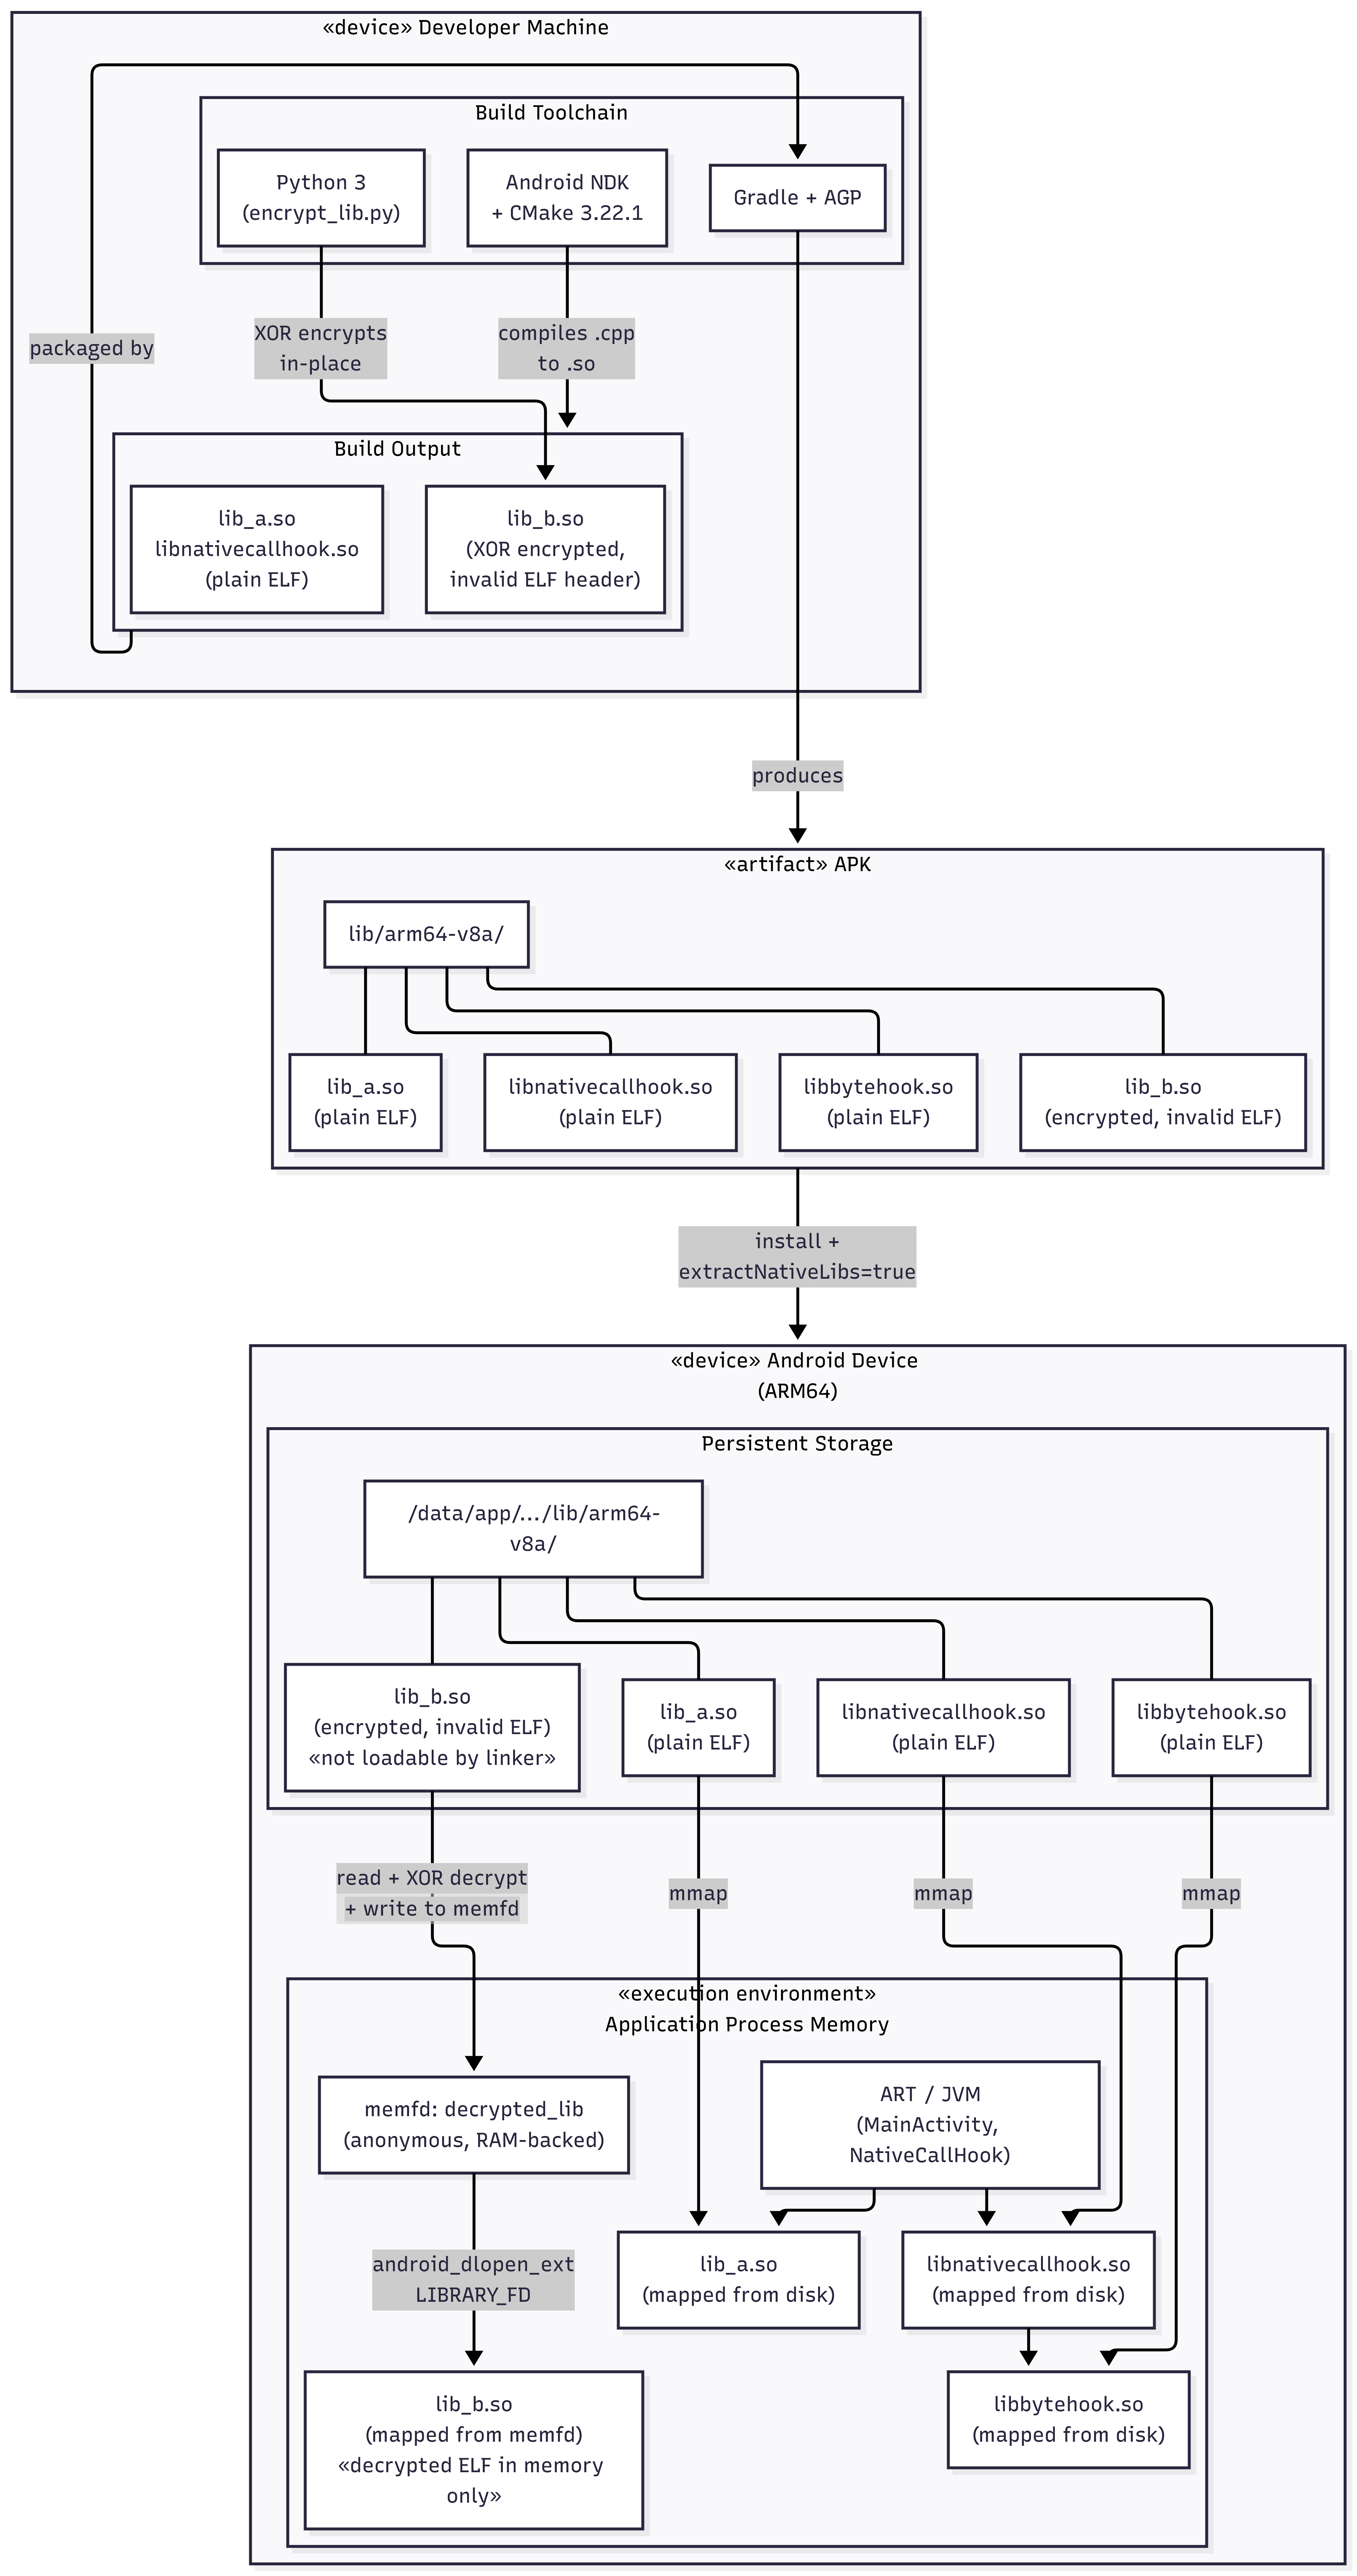
\includegraphics[width=0.7\textwidth]{images/deployment.png}
    \caption{Deployment diagram showing artifact distribution and runtime memory layout.}
    \label{fig:deployment_diagram}
\end{figure}

\subsection{Build-time encryption implementation}

Before packaging, selected native libraries are encrypted so they cannot be mapped by the standard linker.  The encryption step runs inside the CMake build and requires no manual intervention.

\subsubsection{Encryption tool design and implementation}

The encryption tool is a Python script (\texttt{encrypt\_lib.py}) placed alongside the native sources in \texttt{app/src/main/cpp}. CMake invokes it automatically as a post-build step on every incremental or clean build.

A byte-level XOR cipher was chosen deliberately for this prototype. XOR keeps the encryption and decryption code trivial (a single loop over a byte array), which avoids obscuring the more novel contribution of the thesis: the interception, routing, and in-memory loading pipeline. The key, \texttt{0x69}, is a compile-time constant shared between the script and \texttt{nativecallhook.cpp}. In production, this would be replaced with a proper cipher and externalized key management; here it is sufficient to invalidate the on-disk ELF.

Concretely, the script opens the compiled \texttt{.so} binary, XORs every byte with the key, and writes the result back over the original file. After this step, the first four bytes of the library change from the ELF magic \texttt{7f 45 4c 46} to \texttt{16 2c 25 2f}, which is not recognized by any loader. If the Android bionic linker attempts to map the file, it will reject it at the magic-byte check. This property is verifiable with a hex dump of the build artifact and forms the basis of requirement SR1 (no valid protected libraries on disk).

For this prototype, only \texttt{liblibb.so} is encrypted. Its name is hardcoded in the script. A configurable list, read from a file or a Gradle property, would be the natural extension for multi-library scenarios.

\subsubsection{Integration with the build system}

Encryption must happen after linking but before APK packaging. The \texttt{CMakeLists.txt} for the demo application attaches a \texttt{add\_custom\_command(POST\_BUILD ...)} to the \texttt{libb} target, so the script runs in the same directory where the linker emits \texttt{liblibb.so}. No absolute paths are necessary; the working directory is set to \texttt{\$\{CMAKE\_LIBRARY\_OUTPUT\_DIRECTORY\}}, making the step portable across host OSes.

Because the file is encrypted in place, the Gradle packaging stage simply collects the already-encrypted artifact from the CMake output and places it under \texttt{lib/<abi>/} in the APK. No Gradle task modifications or additional packaging rules are needed.

\subsection{Runtime hook initialization}

Hooks must be active before any protected library is requested. On Android, Java code can call \texttt{System.loadLibrary()} at arbitrary points after class loading, so the interception logic needs a launch point that is guaranteed to fire earlier. ELF constructor functions, which the bionic linker executes immediately after mapping a shared object and before returning control to the caller, satisfy this requirement.

\subsubsection{C++ constructor attribute and execution timing}

Marking a function with \texttt{\_\_attribute\_\_((constructor))} places its address in the \texttt{.init\_array} section of the compiled ELF binary. When the dynamic linker finishes loading \texttt{libnativecallhook.so} (via \texttt{System.loadLibrary("nativecallhook")} in Java), it walks the \texttt{.init\_array} and calls each entry before returning to the JVM. Consequently, the constructor runs before \texttt{JNI\_OnLoad} and before any subsequent \texttt{dlopen()} or \texttt{System.loadLibrary()} call the application may issue.

In \texttt{nativecallhook.cpp} the hook-installation logic resides in a static function called \texttt{init\_hook()}, annotated with the constructor attribute. Static linkage limits its symbol visibility to the translation unit, preventing accidental external calls.

\subsubsection{ByteHook framework initialization}

Inside \texttt{init\_hook()}, the first call is \texttt{bytehook\_init(BYTEHOOK\_MODE\_AUTOMATIC, true)}.  The automatic mode tells ByteHook to propagate hooks to shared objects loaded after the initial installation, which is essential because protected libraries have not yet been loaded at this point.  The second argument enables debug-mode output; a release build should pass \texttt{false}.

If the return value signals failure (non-zero), the constructor logs the error and exits immediately, leaving the protection layer disabled.  The application continues to run, but encrypted libraries will not decrypt; this is a deliberate fail-safe.

\subsubsection{Hook installation on the loader entry point}

After ByteHook is ready, \texttt{init\_hook()} installs the interception on \texttt{\_\_loader\_dlopen}, an internal bionic symbol that backs both \texttt{dlopen()} and \texttt{android\_dlopen\_ext()}.  Hooking at this depth, rather than at the public \texttt{dlopen()} wrapper, captures loads that bypass the public API.

The call \texttt{bytehook\_hook\_all(nullptr, "\_\_loader\_dlopen", (void*)hooked\_dlopen, nullptr, nullptr)} instructs ByteHook to patch every PLT entry referencing \texttt{\_\_loader\_dlopen} across all loaded modules.  The first \texttt{nullptr} means no caller-side filter (all callers are intercepted).  The replacement target is the callback \texttt{hooked\_dlopen()}, which is described in \cref{sec:routing}.  The two trailing \texttt{nullptr} arguments disable the optional event callback and user-data pointer, neither of which is needed here.

A non-null return value is the hook stub handle; the implementation stores it globally but does not use it for unhooking in this prototype.  A null return indicates failure; the constructor logs the issue and returns, leaving encrypted libraries unloadable rather than crashing.

\subsection{Protected library registry and routing logic}
\label{sec:routing}

Every native \texttt{dlopen()} call now passes through \texttt{hooked\_dlopen()}.  A lightweight lookup decides whether the request targets a protected library or an ordinary one.

\subsubsection{Registry implementation}

A static \texttt{const char*} array named \texttt{ENCRYPTED\_LIBS} in \texttt{nativecallhook.cpp} lists the protected filenames.  In the prototype, the sole entry is \texttt{"liblibb.so"}.  Hardcoding simplifies the proof of concept but means that each change requires recompilation (a limitation discussed in \cref{sec:routing_limits}).

\subsubsection{Routing decision}

\texttt{hooked\_dlopen()} calls \texttt{is\_encrypted\_library()}, which scans \texttt{ENCRYPTED\_LIBS} with \texttt{strstr()}.  Substring matching was chosen because the dynamic linker may supply the library name as a bare filename, a relative path, or an absolute path; \texttt{strstr()} covers all three forms without path normalization.

When a match is found, \texttt{get\_library\_full\_path()} resolves the on-disk location by invoking \texttt{dladdr()} on the calling library to discover the extracted-libraries directory, and passes the result to \texttt{load\_decrypted\_library()}.  When no match is found, \texttt{BYTEHOOK\_CALL\_PREV} forwards the request to the original \texttt{\_\_loader\_dlopen}, giving unprotected libraries zero additional overhead.

Path resolution assumes \texttt{android:extractNativeLibs="true"}, meaning all \texttt{.so} files reside in a single directory under \texttt{/data/app/}.

\subsubsection{Limitations}
\label{sec:routing_limits}

The hardcoded registry prevents runtime configuration.  A production variant should read the protected-library list from a resource or receive it through a JNI registration call.  The current registry stores filenames only, with no integrity hashes or per-library key identifiers.  \texttt{strstr()} matching can also produce false positives when one library name is a substring of another (e.g.\ \texttt{liblibb.so} would match \texttt{liblibb\_v2.so}).

\subsection{In-memory decryption and loading}

When the routing logic identifies a protected library, \texttt{load\_decrypted\_library()} decrypts it and maps it into the process entirely in memory.  The function performs five discrete operations: file read, XOR decryption, ELF magic-byte validation, anonymous file-descriptor creation, and linker invocation.

\subsubsection{Reading and decrypting the encrypted library}

\texttt{get\_library\_full\_path()} supplies the absolute path to the encrypted \texttt{.so} under \texttt{/data/app/}.  The file is read into a \texttt{std::vector<uint8\_t>} in a single I/O pass; this buffer will be discarded after the decrypted content is written to the anonymous descriptor, limiting the window during which plaintext exists in heap memory.

Decryption is a byte-wise XOR with the same key (\texttt{0x69}) used at build time.  XOR is its own inverse, so no separate decryption routine is needed.

\subsubsection{ELF validation}

Before attempting to load, the function checks bytes 0--3 of the decrypted buffer against the ELF magic sequence \texttt{0x7f 0x45 0x4c 0x46}.  A mismatch means the wrong key was applied, the file was corrupted, or it was tampered with.  In each case, the function returns \texttt{nullptr} without calling the linker, satisfying the fail-safe requirement that malformed images must never execute.

\subsubsection{Anonymous file descriptor creation with memfd\_create}

\texttt{memfd\_create()} (Linux syscall \texttt{\_\_NR\_memfd\_create}, available since kernel 3.17 / Android API 26) returns a file descriptor backed exclusively by RAM.  The call uses \texttt{MFD\_CLOEXEC} so the descriptor is not inherited by child processes.

After creation, \texttt{ftruncate()} sizes the descriptor to the buffer length and \texttt{write()} copies the decrypted bytes into it.  A failed \texttt{memfd\_create()} (possible under extreme memory pressure or restrictive seccomp filters) causes the function to log the \texttt{errno} value and return \texttt{nullptr}.

\subsubsection{Loading via android\_dlopen\_ext}

\texttt{android\_dlopen\_ext()} \cite{android_ndk_dlext} extends the standard \texttt{dlopen()} interface with an \texttt{android\_dlextinfo} structure.  Setting the \texttt{ANDROID\_DLEXT\_USE\_LIBRARY\_FD} flag and populating the \texttt{library\_fd} field directs the bionic linker to read ELF segments from the memfd rather than opening a path on disk.  The linker maps segments, resolves relocations, processes dependencies, and executes \texttt{.init\_array} constructors in the normal way; the calling code receives a standard \texttt{void*} handle compatible with \texttt{dlsym()}.

On success, the memfd descriptor is kept open for the lifetime of the loaded library because the linker may hold memory-mapped regions that reference it.  On failure, the descriptor is closed and \texttt{nullptr} is returned.  The heap buffer is freed immediately after the \texttt{write()} call in either case.

\subsubsection{Security implications}

The plaintext library exists only inside the process address space: first briefly in a heap buffer, then as linker-mapped pages backed by the anonymous descriptor.  No plaintext ever reaches persistent storage, satisfying requirement SR2.

An attacker who can attach a debugger or read \texttt{/proc/<pid>/mem} could still dump the decrypted image.  The prototype does not implement anti-debugging, memory sealing, or obfuscation.  These countermeasures are out of scope for the proof of concept but would be necessary in a hardened deployment.

\subsection{Java-Native integration and load order}

Correct load sequencing is essential: hooks must be installed before any code, Java or native, requests a protected library.

\subsubsection{Load order enforcement}

\texttt{NativeCallHook} declares a Java \texttt{static} block that calls \texttt{System.loadLibrary("nativecallhook")}, which triggers the C++ constructor described in the previous section.  \texttt{MainActivity} enforces ordering in its own static block by calling \texttt{NativeCallHook.initialize()} first, then \texttt{System.loadLibrary("liba")}.  Because the JVM executes static initializers exactly once and in declaration order, hooks are guaranteed to be active before the application's own native code runs.

\subsubsection{Native-to-native loading validation}

The demo validates nested loading through \texttt{loadEncryptedLibrary()}, a JNI method in \texttt{liba} that internally calls \texttt{dlopen("liblibb.so", ...)} and \texttt{dlsym()} to resolve and invoke a function.  Because \texttt{liblibb.so} appears in the encrypted-library registry, the PLT hook intercepts the \texttt{dlopen()} call, decrypts the file from disk, and returns a valid handle, all entirely transparently to the caller.  From \texttt{liba}'s perspective, the load is indistinguishable from an ordinary \texttt{dlopen()} of an unprotected library.

\subsubsection{JNI bridge}

\texttt{jni\_bridge.cpp} exposes three native methods to the Java layer: \texttt{initialize()} (returns \texttt{JNI\_TRUE} to confirm hook installation), \texttt{getStatus()} (returns a status string), and \texttt{log()} (writes to Logcat through the native layer).  \texttt{JNI\_OnLoad()} is present only to satisfy the JNI protocol and logs a confirmation message; no initialization work occurs there because the constructor has already completed.

\newpage

\subsection{System testing}

The following tests were run on a physical Google Pixel 9 device connected via USB and accessed through ADB. All tests use the debug build compiled for \texttt{arm64-v8a}. Logcat output is filtered by the tag \texttt{NATIVECALLHOOK}, which all native and Java components share.

\begin{table}[h]
\centering
\caption{Test device and software configuration.}
\label{tab:test_env}
\begin{tabular}{l l}
    \hline
    \textbf{Parameter} & \textbf{Value} \\
    \hline
    Device & Google Pixel 9 \\
    Android version & 16 (API level 36) \\
    Build ID & CP1A.260305.018 \\
    Security patch & 2026-03-05 \\
    ABI & arm64-v8a \\
    Kernel & 6.1.145-android14-11 \\
    Build type & Debug (debuggable, JNI debuggable) \\
    \hline
\end{tabular}
\end{table}

\subsubsection{Build-time encryption verification}

The first check was to confirm that \texttt{liblibb.so} inside the installed APK is not a valid ELF binary (SR1). The first 16 bytes of three installed libraries were read using \texttt{xxd} via ADB:

\begin{verbatim}
libliba.so  (unprotected):
  00000000: 7f45 4c46 0201 0100 0000 0000 0000 0000

liblibb.so  (encrypted):
  00000000: 162c 252f 6b68 6869 6969 6969 6969 6969

libnativecallhook.so  (hook library):
  00000000: 7f45 4c46 0201 0100 0000 0000 0000 0000
\end{verbatim}

\texttt{libliba.so} and \texttt{libnativecallhook.so} carry the standard ELF magic \texttt{7f 45 4c 46}. \texttt{liblibb.so} begins with \texttt{16 2c 25 2f}, which is \texttt{7f 45 4c 46} XOR \texttt{0x69}. The bionic linker checks those first four bytes before parsing anything else; since the sequence is unrecognized, any direct load attempt is rejected immediately. SR1 is satisfied.

\subsubsection{Hook installation}

To verify that \texttt{init\_hook()} runs before the rest of the application, the demo app was launched from a cold start and the Logcat output was captured:

\begin{verbatim}
18:46:42.656 I NATIVECALLHOOK: dlopen hook installed successfully
18:46:42.692 I NATIVECALLHOOK: NativeCallHook active — hooks installed
18:46:42.692 I NATIVECALLHOOK: MainActivity started
\end{verbatim}

The hook confirmation at 42.656 precedes both the \texttt{JNI\_OnLoad} status message and the first \texttt{MainActivity} log line. \texttt{bytehook\_hook\_all()} returned a valid stub handle, meaning the PLT entries for \texttt{\_\_loader\_dlopen} were patched process-wide before any subsequent library load could take place. FR1 is satisfied.

\subsubsection{Unprotected library passthrough}

The same Logcat session was examined for any interception line mentioning \texttt{liba}. None were found. The only interception entry in the entire session is:

\begin{verbatim}
18:46:42.692 I NATIVECALLHOOK: Intercepted dlopen for encrypted
  library: liblibb.so
\end{verbatim}

\texttt{libliba.so} loaded via \texttt{System.loadLibrary()} and was forwarded through \texttt{BYTEHOOK\_CALL\_\allowbreak PREV} directly to the original loader unchanged. The hook adds no overhead to libraries that are not in the protected registry. FR3 is satisfied.

\subsubsection{Protected library end-to-end load}

The core decryption pipeline was verified by capturing the lines that \texttt{load\_decrypted\_library()} emits at each stage:

\begin{verbatim}
18:46:42.692 I NATIVECALLHOOK: Intercepted dlopen for encrypted
  library: liblibb.so
18:46:42.692 I NATIVECALLHOOK: Loading encrypted library:
  /data/app/.../lib/arm64/liblibb.so
18:46:42.694 I NATIVECALLHOOK: Successfully loaded decrypted
  library from memfd
\end{verbatim}

Interception, file read, XOR decryption, ELF magic validation, \texttt{memfd\_create}, and \texttt{android\_dlopen\_\allowbreak ext()} all completed without error. No ``Invalid ELF'' message appeared, confirming the decrypted bytes passed the magic-byte check. The 2\,ms gap between the first and last entries reflects the file I/O and decryption time for the small test library. Requirements FR2, SR2, and SR3 are satisfied.

\subsubsection{Native-to-native load coverage}

This test confirms the central claim of the thesis: a native library can transparently load a protected native library through an intercepted \texttt{dlopen()} call. The \texttt{loadEncryptedLibrary()} JNI method in \texttt{liba} issues \texttt{dlopen("liblibb.so")} with \texttt{RTLD\_LAZY}, resolves \texttt{call\_logcat} with \texttt{dlsym()}, and calls it. The resulting output was:

\begin{verbatim}
18:46:42.694 I NATIVECALLHOOK: LibB: Hello from LibB,
  called by LibA after decryption
\end{verbatim}

\texttt{call\_logcat()} inside the decrypted \texttt{liblibb.so} executed correctly. The \texttt{dlopen()} call from within \texttt{liba} was intercepted, the library was decrypted and loaded through the memfd path, and the returned handle was valid for \texttt{dlsym()}. From \texttt{liba}'s perspective, the operation is indistinguishable from loading an ordinary shared object. FR4 is satisfied.

\subsubsection{Fail-safe behaviour}

To test the ELF validation path, the \texttt{XOR\_KEY} constant in \texttt{nativecallhook.cpp} was changed from \texttt{0x69} to \texttt{0xAA}, the APK was rebuilt and reinstalled, and the app was launched:

\begin{verbatim}
18:46:58.531 I NATIVECALLHOOK: dlopen hook installed successfully
18:46:58.563 I NATIVECALLHOOK: Intercepted dlopen for encrypted
  library: liblibb.so
18:46:58.563 I NATIVECALLHOOK: Loading encrypted library:
  /data/app/.../lib/arm64/liblibb.so
18:46:58.564 E NATIVECALLHOOK: Invalid ELF magic after decryption
18:46:58.564 E NATIVECALLHOOK: LibA: Failed to load LibB
\end{verbatim}

Decrypting with the wrong key produced bytes that did not begin with \texttt{7f 45 4c 46}. \texttt{load\_decrypted\_\allowbreak library()} returned \texttt{nullptr} without invoking the linker, and no fallback to the original encrypted file was attempted. The application process (PID~11415) remained alive, confirming that a failed protected-library load is non-fatal. After data collection, the original key was restored and the correct APK was reinstalled. SR4 is satisfied.

\subsubsection{Load order enforcement}

The final test demonstrates that the static block ordering in \texttt{MainActivity} is functionally significant, not just a convention. A test build was prepared with two changes: an \texttt{\_\_attribute\_\_\allowbreak((constructor))} function was added to \texttt{lib\_a.cpp} that calls \texttt{dlopen("liblibb.so")} during \texttt{System.\allowbreak loadLibrary("liba")}, and the static block was reordered so that \texttt{System.\allowbreak loadLibrary("liba")} ran before \texttt{NativeCallHook.\allowbreak initialize()}.

\begin{verbatim}
18:49:43.168 I NATIVECALLHOOK: LibA constructor: attempting
  dlopen("liblibb.so")
18:49:43.168 E NATIVECALLHOOK: LibA constructor: dlopen failed:
  ".../liblibb.so" has bad ELF magic: 162c252f
18:49:43.189 I NATIVECALLHOOK: dlopen hook installed successfully
18:49:43.222 I NATIVECALLHOOK: Intercepted dlopen for encrypted
  library: liblibb.so
18:49:43.223 I NATIVECALLHOOK: Successfully loaded decrypted
  library from memfd
18:49:43.223 I NATIVECALLHOOK: LibB: Hello from LibB,
  called by LibA after decryption
\end{verbatim}

At 43.168 the \texttt{liba} constructor ran before hook installation at 43.189. The bionic linker received the encrypted file directly, read the first four bytes as \texttt{162c252f}, and rejected it. Eighteen milliseconds later the hook was installed and the \texttt{loadEncryptedLibrary()} call from \texttt{onCreate()} at 43.222 succeeded normally. Both source files were reverted and the correct APK was reinstalled after the test. This confirms that the protection library must be initialized before any code that may request a protected library.

\subsubsection{Summary of test results}

All seven tests passed on the Google Pixel 9 running Android~16. The results are mapped to the relevant requirements in \cref{tab:test_results}.

\begin{table}[h]
\centering
\caption{Test results mapped to system requirements.}
\label{tab:test_results}
\begin{tabular}{l l l l}
    \hline
    \textbf{Test} & \textbf{Requirement} & \textbf{Observed result} & \textbf{Status} \\
    \hline
    Build-time encryption & SR1 & Invalid ELF on disk confirmed & Pass \\
    Hook installation & FR1 & Hook active before first load & Pass \\
    Unprotected passthrough & FR3 & No false interceptions & Pass \\
    Protected end-to-end load & FR2, SR2, SR3 & Decrypt and memfd load & Pass \\
    Native-to-native coverage & FR4 & \texttt{dlopen} chain works & Pass \\
    Fail-safe behaviour & SR4 & Invalid ELF rejected cleanly & Pass \\
    Load order enforcement & FR1 & Early load fails without hook & Pass \\
    \hline
\end{tabular}
\end{table}

The test set covers all four security requirements and the functional requirements directly tied to the thesis objective. The results show that the interception, decryption, and in-memory loading pipeline operates correctly on a stock Android~16 device and that the system behaves safely when given incorrect input or when initialization order is violated.

\newpage

\section*{Conclusions}
\addcontentsline{toc}{section}{Conclusions}

This thesis addressed the limitation of conventional Android native library protection approaches that only cover managed-code initiated loading and do not reliably handle nested native-to-native loading scenarios. A proof-of-concept protection mechanism was designed and implemented to ensure that selected native libraries remain encrypted on disk and are only decrypted inside the target process immediately before loading.

\begin{enumerate}
    \item The analysis of Android native library loading, ELF dynamic linking, and interception methods showed that Java-level hooking mechanisms cannot fully observe or control library loads initiated from native code, motivating the need for native interception at the dynamic linker boundary.
    \item A proof-of-concept system architecture was defined that combines a build-time encryption step with a runtime interception component, while preserving standard Android packaging and installation behaviour by keeping encrypted libraries in the normal APK native library locations.
    \item The runtime protection component was implemented using PLT-based interception to route native loading requests through a registry-driven decision mechanism, enabling transparent handling of both protected and unprotected libraries with a strict fail-safe policy when protected library loading fails.
    \item Protected libraries were loaded by decrypting encrypted on-disk content into memory, creating an anonymous in-memory file descriptor, and invoking the Android extended loader interface to map the decrypted ELF image into the process without writing plaintext content to persistent storage.
    \item The proof-of-concept validated correct load order enforcement and demonstrated transparent nested native-to-native loading in the demo scenario, confirming that intercepted \texttt{dlopen()} calls from within native libraries can be routed through the decryption and in-memory loading path.
\end{enumerate}

The implemented solution is intentionally limited by proof-of-concept design choices, including a hardcoded protected library registry and a simple XOR-based encryption scheme with a hardcoded key. In future work, the system should introduce stronger cryptography and secure key management (for example, Android Keystore-backed derivation), make the protected library registry configurable at build time or runtime, add integrity verification of decrypted images, and provide a quantitative evaluation of performance overhead and compatibility across a broader set of Android versions, devices, and packaging configurations.


% ============================================================================
% REFERENCES
% ============================================================================
\renewcommand{\bibname}{References}
\begin{thebibliography}{99}

\bibitem{appfigures2024flutter}
Appfigures.
\textit{Non-Native Development Trends - Will React Native's New Architecture Take the Lead Away from Flutter?}
2024 [žiūrėta 2025-10-20].
Prieiga per internetą:
\url{https://appfigures.com/resources/insights/20241025}

\bibitem{android_platform}
Android Developers.
\textit{Platform architecture.}
2025 [žiūrėta 2025-10-20].
Prieiga per internetą:
\url{https://developer.android.com/guide/platform}

\bibitem{xinuos2025elf}
Xinuos Inc.
\textit{System V Application Binary Interface – Executable and Linking Format (ELF) Specification Version 4.3 Draft.}
2025 [žiūrėta 2025-10-27].
Prieiga per internetą:
\url{https://gabi.xinuos.com/}

\bibitem{ronin2018hooking}
N. Totosis and C. Patsakis.
\textit{Android Hooking Revisited.}
2018.
doi: \href{https://doi.org/10.1109/DASC/PiCom/DataCom/CyberSciTec.2018.00104}{10.1109/DASC/PiCom/DataCom/CyberSciTec.2018.00104}

\bibitem{bleier2023oat}
J. Bleier and M. Lindorfer.
\textit{Of Ahead Time: Evaluating Disassembly of Android Apps Compiled to Binary OATs Through the ART.}
2023 [žiūrėta 2025-10-26].
Prieiga per internetą:
\url{https://repositum.tuwien.at/bitstream/20.500.12708/190032/3/Bleier-2023-Of%20Ahead%20Time%20Evaluating%20Disassembly%20of%20Android%20Apps%20Compiled...-vor.pdf}
doi: \href{https://doi.org/10.1145/3578357.3591219}{10.1145/3578357.3591219}

\bibitem{xposed2013framework}
rovo89.
\textit{Xposed Framework} [software].
XDA-Developers, 2013 [žiūrėta 2025-10-26].
Prieiga per internetą:
\url{https://forum.xda-developers.com/t/xposed-framework.2327541/}

\bibitem{kumar2023inviseal}
S. Kumar, D. Mishra, B. Panda, and S. K. Shukla.
\textit{InviSeal: A Stealthy Dynamic Analysis Framework for Android Systems.}
2023.
doi: \href{https://doi.org/10.1145/3567599}{10.1145/3567599}

\bibitem{frida2023official}
O. A. Ravnås.
\textit{Frida – Dynamic instrumentation toolkit for developers, reverse-engineers, and security researchers.}
2023 [žiūrėta 2025-10-26].
Prieiga per internetą:
\url{https://frida.re}

\bibitem{pizzi2022virtualpatch}
S. Pizzi.
\textit{VirtualPatch: fixing Android security vulnerabilities with app-level virtualization.}
Magistro baigiamasis darbas, Università degli Studi di Padova, 2022 [žiūrėta 2025-11-16].
Prieiga per internetą:
\url{https://thesis.unipd.it/bitstream/20.500.12608/32823/1/Pizzi_Simeone.pdf}

\bibitem{lsposed2025github}
JingMatrix.
\textit{Vector (formerly LSPosed Framework).}
GitHub repository, 2025 [žiūrėta 2025-11-16].
Prieiga per internetą:
\url{https://github.com/JingMatrix/Vector}

\bibitem{lsposed2025website}
LSPosed Team.
\textit{LSPosed Official Website.}
2025 [žiūrėta 2025-11-16].
Prieiga per internetą:
\url{https://lsposed.org}

\bibitem{androidroot2024lsposed}
Awesome Android Root.
\textit{Complete LSPosed Framework Guide.}
2024 [žiūrėta 2025-11-16].
Prieiga per internetą:
\url{https://awesome-android-root.org/rooting-guides/lsposed-guide}

\bibitem{promon2024hooking}
Promon AS.
\textit{Mobile app security basics: Understanding hooking frameworks and hooking techniques.}
2024 [žiūrėta 2025-11-16].
Prieiga per internetą:
\url{https://promon.io/resources/knowledge-center/hooking-framework-hooking-techniques}

\bibitem{bytehook2025github}
ByteDance.
\textit{ByteHook – Android PLT hook library.}
GitHub, 2025 [žiūrėta 2025-11-16].
Prieiga per internetą:
\url{https://github.com/bytedance/bhook}

\bibitem{bytehook2025maven}
Sonatype.
\textit{com.bytedance:bytehook – ByteHook is an Android PLT hook library which supports armeabi-v7a, arm64-v8a, x86 and x86\_64.}
Maven Central, 2025 [žiūrėta 2025-11-16].
Prieiga per internetą:
\url{https://central.sonatype.com/artifact/com.bytedance/bytehook}

\bibitem{android_ndk_dlext}
Android Developers.
\textit{\textless android/dlext.h\textgreater{} -- Android NDK Reference.}
2025 [žiūrėta 2025-11-16].
Prieiga per internetą:
\url{https://developer.android.com/ndk/reference/group/libdl}

\end{thebibliography}



\end{document}
